
%% bare_jrnl.tex
%% V1.4b
%% 2015/08/26
%% by Michael Shell
%% see http://www.michaelshell.org/
%% for current contact information.
%%
%% This is a skeleton file demonstrating the use of IEEEtran.cls
%% (requires IEEEtran.cls version 1.8b or later) with an IEEE
%% journal paper.
%%
%% Support sites:
%% http://www.michaelshell.org/tex/ieeetran/
%% http://www.ctan.org/pkg/ieeetran
%% and
%% http://www.ieee.org/

%%*************************************************************************
%% Legal Notice:
%% This code is offered as-is without any warranty either expressed or
%% implied; without even the implied warranty of MERCHANTABILITY or
%% FITNESS FOR A PARTICULAR PURPOSE! 
%% User assumes all risk.
%% In no event shall the IEEE or any contributor to this code be liable for
%% any damages or losses, including, but not limited to, incidental,
%% consequential, or any other damages, resulting from the use or misuse
%% of any information contained here.
%%
%% All comments are the opinions of their respective authors and are not
%% necessarily endorsed by the IEEE.
%%
%% This work is distributed under the LaTeX Project Public License (LPPL)
%% ( http://www.latex-project.org/ ) version 1.3, and may be freely used,
%% distributed and modified. A copy of the LPPL, version 1.3, is included
%% in the base LaTeX documentation of all distributions of LaTeX released
%% 2003/12/01 or later.
%% Retain all contribution notices and credits.
%% ** Modified files should be clearly indicated as such, including  **
%% ** renaming them and changing author support contact information. **
%%*************************************************************************


% *** Authors should verify (and, if needed, correct) their LaTeX system  ***
% *** with the testflow diagnostic prior to trusting their LaTeX platform ***
% *** with production work. The IEEE's font choices and paper sizes can   ***
% *** trigger bugs that do not appear when using other class files.       ***                          ***
% The testflow support page is at:
% http://www.michaelshell.org/tex/testflow/



\documentclass[journal]{IEEEtran}
%
% If IEEEtran.cls has not been installed into the LaTeX system files,
% manually specify the path to it like:
% \documentclass[journal]{../sty/IEEEtran}





% Some very useful LaTeX packages include:
% (uncomment the ones you want to load)


% *** MISC UTILITY PACKAGES ***
%
%\usepackage{ifpdf}
% Heiko Oberdiek's ifpdf.sty is very useful if you need conditional
% compilation based on whether the output is pdf or dvi.
% usage:
% \ifpdf
%   % pdf code
% \else
%   % dvi code
% \fi
% The latest version of ifpdf.sty can be obtained from:
% http://www.ctan.org/pkg/ifpdf
% Also, note that IEEEtran.cls V1.7 and later provides a builtin
% \ifCLASSINFOpdf conditional that works the same way.
% When switching from latex to pdflatex and vice-versa, the compiler may
% have to be run twice to clear warning/error messages.






% *** CITATION PACKAGES ***
%
%\usepackage{cite}
% cite.sty was written by Donald Arseneau
% V1.6 and later of IEEEtran pre-defines the format of the cite.sty package
% \cite{} output to follow that of the IEEE. Loading the cite package will
% result in citation numbers being automatically sorted and properly
% "compressed/ranged". e.g., [1], [9], [2], [7], [5], [6] without using
% cite.sty will become [1], [2], [5]--[7], [9] using cite.sty. cite.sty's
% \cite will automatically add leading space, if needed. Use cite.sty's
% noadjust option (cite.sty V3.8 and later) if you want to turn this off
% such as if a citation ever needs to be enclosed in parenthesis.
% cite.sty is already installed on most LaTeX systems. Be sure and use
% version 5.0 (2009-03-20) and later if using hyperref.sty.
% The latest version can be obtained at:
% http://www.ctan.org/pkg/cite
% The documentation is contained in the cite.sty file itself.






% *** GRAPHICS RELATED PACKAGES ***
%
\ifCLASSINFOpdf
  \usepackage[pdftex]{graphicx}
  \usepackage{bm}
  \usepackage{amsfonts}
  \usepackage{amsmath}
  \usepackage{multirow}
  \usepackage{color}

  \newcommand{\dlt}[1]{}
  \newcommand{\cxj}[1]{\textcolor{red}{(#1)}}
  \newcommand{\rpl}[1]{\textcolor{yellow}{(#1)}}
  \newcommand{\mdf}[1]{\textcolor{blue}{#1}}
  \newcommand{\vset}[1]{#1_{1:T}} %% denote for the input frames 
  \newcommand{\msset}[1]{\{#1_{t-7},#1_{t-3},#1_{t},#1_{t+3},#1_{t+7}\}}
  \newcommand{\gtframe}{\widetilde{Y}_t} %% denote for the ground truthe frame Y_t 
  % declare the path(s) where your graphic files are
  % \graphicspath{{../pdf/}{../jpeg/}}
  % and their extensions so you won't have to specify these with
  % every instance of \includegraphics
  % \DeclareGraphicsExtensions{.pdf,.jpeg,.png}
\else
  % or other class option (dvipsone, dvipdf, if not using dvips). graphicx
  % will default to the driver specified in the system graphics.cfg if no
  % driver is specified.
  % \usepackage[dvips]{graphicx}
  % declare the path(s) where your graphic files are
  % \graphicspath{{../eps/}}
  % and their extensions so you won't have to specify these with
  % every instance of \includegraphics
  % \DeclareGraphicsExtensions{.eps}
\fi
% graphicx was written by David Carlisle and Sebastian Rahtz. It is
% required if you want graphics, photos, etc. graphicx.sty is already
% installed on most LaTeX systems. The latest version and documentation
% can be obtained at: 
% http://www.ctan.org/pkg/graphicx
% Another good source of documentation is "Using Imported Graphics in
% LaTeX2e" by Keith Reckdahl which can be found at:
% http://www.ctan.org/pkg/epslatex
%
% latex, and pdflatex in dvi mode, support graphics in encapsulated
% postscript (.eps) format. pdflatex in pdf mode supports graphics
% in .pdf, .jpeg, .png and .mps (metapost) formats. Users should ensure
% that all non-photo figures use a vector format (.eps, .pdf, .mps) and
% not a bitmapped formats (.jpeg, .png). The IEEE frowns on bitmapped formats
% which can result in "jaggedy"/blurry rendering of lines and letters as
% well as large increases in file sizes.
%
% You can find documentation about the pdfTeX application at:
% http://www.tug.org/applications/pdftex





% *** MATH PACKAGES ***
%
%\usepackage{amsmath}
% A popular package from the American Mathematical Society that provides
% many useful and powerful commands for dealing with mathematics.
%
% Note that the amsmath package sets \interdisplaylinepenalty to 10000
% thus preventing page breaks from occurring within multiline equations. Use:
%\interdisplaylinepenalty=2500
% after loading amsmath to restore such page breaks as IEEEtran.cls normally
% does. amsmath.sty is already installed on most LaTeX systems. The latest
% version and documentation can be obtained at:
% http://www.ctan.org/pkg/amsmath





% *** SPECIALIZED LIST PACKAGES ***
%
%\usepackage{algorithmic}
% algorithmic.sty was written by Peter Williams and Rogerio Brito.
% This package provides an algorithmic environment fo describing algorithms.
% You can use the algorithmic environment in-text or within a figure
% environment to provide for a floating algorithm. Do NOT use the algorithm
% floating environment provided by algorithm.sty (by the same authors) or
% algorithm2e.sty (by Christophe Fiorio) as the IEEE does not use dedicated
% algorithm float types and packages that provide these will not provide
% correct IEEE style captions. The latest version and documentation of
% algorithmic.sty can be obtained at:
% http://www.ctan.org/pkg/algorithms
% Also of interest may be the (relatively newer and more customizable)
% algorithmicx.sty package by Szasz Janos:
% http://www.ctan.org/pkg/algorithmicx




% *** ALIGNMENT PACKAGES ***
%
%\usepackage{array}
% Frank Mittelbach's and David Carlisle's array.sty patches and improves
% the standard LaTeX2e array and tabular environments to provide better
% appearance and additional user controls. As the default LaTeX2e table
% generation code is lacking to the point of almost being broken with
% respect to the quality of the end results, all users are strongly
% advised to use an enhanced (at the very least that provided by array.sty)
% set of table tools. array.sty is already installed on most systems. The
% latest version and documentation can be obtained at:
% http://www.ctan.org/pkg/array


% IEEEtran contains the IEEEeqnarray family of commands that can be used to
% generate multiline equations as well as matrices, tables, etc., of high
% quality.




% *** SUBFIGURE PACKAGES ***
%\ifCLASSOPTIONcompsoc
%  \usepackage[caption=false,font=normalsize,labelfont=sf,textfont=sf]{subfig}
%\else
%  \usepackage[caption=false,font=footnotesize]{subfig}
%\fi
% subfig.sty, written by Steven Douglas Cochran, is the modern replacement
% for subfigure.sty, the latter of which is no longer maintained and is
% incompatible with some LaTeX packages including fixltx2e. However,
% subfig.sty requires and automatically loads Axel Sommerfeldt's caption.sty
% which will override IEEEtran.cls' handling of captions and this will result
% in non-IEEE style figure/table captions. To prevent this problem, be sure
% and invoke subfig.sty's "caption=false" package option (available since
% subfig.sty version 1.3, 2005/06/28) as this is will preserve IEEEtran.cls
% handling of captions.
% Note that the Computer Society format requires a larger sans serif font
% than the serif footnote size font used in traditional IEEE formatting
% and thus the need to invoke different subfig.sty package options depending
% on whether compsoc mode has been enabled.
%
% The latest version and documentation of subfig.sty can be obtained at:
% http://www.ctan.org/pkg/subfig




% *** FLOAT PACKAGES ***
%
%\usepackage{fixltx2e}
% fixltx2e, the successor to the earlier fix2col.sty, was written by
% Frank Mittelbach and David Carlisle. This package corrects a few problems
% in the LaTeX2e kernel, the most notable of which is that in current
% LaTeX2e releases, the ordering of single and double column floats is not
% guaranteed to be preserved. Thus, an unpatched LaTeX2e can allow a
% single column figure to be placed prior to an earlier double column
% figure.
% Be aware that LaTeX2e kernels dated 2015 and later have fixltx2e.sty's
% corrections already built into the system in which case a warning will
% be issued if an attempt is made to load fixltx2e.sty as it is no longer
% needed.
% The latest version and documentation can be found at:
% http://www.ctan.org/pkg/fixltx2e


%\usepackage{stfloats}
% stfloats.sty was written by Sigitas Tolusis. This package gives LaTeX2e
% the ability to do double column floats at the bottom of the page as well
% as the top. (e.g., "\begin{figure*}[!b]" is not normally possible in
% LaTeX2e). It also provides a command:
%\fnbelowfloat
% to enable the placement of footnotes below bottom floats (the standard
% LaTeX2e kernel puts them above bottom floats). This is an invasive package
% which rewrites many portions of the LaTeX2e float routines. It may not work
% with other packages that modify the LaTeX2e float routines. The latest
% version and documentation can be obtained at:
% http://www.ctan.org/pkg/stfloats
% Do not use the stfloats baselinefloat ability as the IEEE does not allow
% \baselineskip to stretch. Authors submitting work to the IEEE should note
% that the IEEE rarely uses double column equations and that authors should try
% to avoid such use. Do not be tempted to use the cuted.sty or midfloat.sty
% packages (also by Sigitas Tolusis) as the IEEE does not format its papers in
% such ways.
% Do not attempt to use stfloats with fixltx2e as they are incompatible.
% Instead, use Morten Hogholm'a dblfloatfix which combines the features
% of both fixltx2e and stfloats:
%
% \usepackage{dblfloatfix}
% The latest version can be found at:
% http://www.ctan.org/pkg/dblfloatfix




%\ifCLASSOPTIONcaptionsoff
%  \usepackage[nomarkers]{endfloat}
% \let\MYoriglatexcaption\caption
% \renewcommand{\caption}[2][\relax]{\MYoriglatexcaption[#2]{#2}}
%\fi
% endfloat.sty was written by James Darrell McCauley, Jeff Goldberg and 
% Axel Sommerfeldt. This package may be useful when used in conjunction with 
% IEEEtran.cls'  captionsoff option. Some IEEE journals/societies require that
% submissions have lists of figures/tables at the end of the paper and that
% figures/tables without any captions are placed on a page by themselves at
% the end of the document. If needed, the draftcls IEEEtran class option or
% \CLASSINPUTbaselinestretch interface can be used to increase the line
% spacing as well. Be sure and use the nomarkers option of endfloat to
% prevent endfloat from "marking" where the figures would have been placed
% in the text. The two hack lines of code above are a slight modification of
% that suggested by in the endfloat docs (section 8.4.1) to ensure that
% the full captions always appear in the list of figures/tables - even if
% the user used the short optional argument of \caption[]{}.
% IEEE papers do not typically make use of \caption[]'s optional argument,
% so this should not be an issue. A similar trick can be used to disable
% captions of packages such as subfig.sty that lack options to turn off
% the subcaptions:
% For subfig.sty:
% \let\MYorigsubfloat\subfloat
% \renewcommand{\subfloat}[2][\relax]{\MYorigsubfloat[]{#2}}
% However, the above trick will not work if both optional arguments of
% the \subfloat command are used. Furthermore, there needs to be a
% description of each subfigure *somewhere* and endfloat does not add
% subfigure captions to its list of figures. Thus, the best approach is to
% avoid the use of subfigure captions (many IEEE journals avoid them anyway)
% and instead reference/explain all the subfigures within the main caption.
% The latest version of endfloat.sty and its documentation can obtained at:
% http://www.ctan.org/pkg/endfloat
%
% The IEEEtran \ifCLASSOPTIONcaptionsoff conditional can also be used
% later in the document, say, to conditionally put the References on a 
% page by themselves.




% *** PDF, URL AND HYPERLINK PACKAGES ***
%
%\usepackage{url}
% url.sty was written by Donald Arseneau. It provides better support for
% handling and breaking URLs. url.sty is already installed on most LaTeX
% systems. The latest version and documentation can be obtained at:
% http://www.ctan.org/pkg/url
% Basically, \url{my_url_here}.




% *** Do not adjust lengths that control margins, column widths, etc. ***
% *** Do not use packages that alter fonts (such as pslatex).         ***
% There should be no need to do such things with IEEEtran.cls V1.6 and later.
% (Unless specifically asked to do so by the journal or conference you plan
% to submit to, of course. )

\usepackage{multirow}
\usepackage{cmath}
\usepackage{algorithm, algorithmic}
\usepackage{amsmath}
\usepackage{pifont}
\newcommand{\cmark}{\text{\ding{51}}}
\newcommand{\xmark}{\text{\ding{55}}}

% correct bad hyphenation here
\hyphenation{op-tical net-works semi-conduc-tor}


\begin{document}
%
% paper title
% Titles are generally capitalized except for words such as a, an, and, as,
% at, but, by, for, in, nor, of, on, or, the, to and up, which are usually
% not capitalized unless they are the first or last word of the title.
% Linebreaks \\ can be used within to get better formatting as desired.
% Do not put math or special symbols in the title.
\title{Structure-Guided Deep Video Inpainting}
%
%
% author names and IEEE memberships
% note positions of commas and nonbreaking spaces ( ~ ) LaTeX will not break
% a structure at a ~ so this keeps an author's name from being broken across
% two lines.
% use \thanks{} to gain access to the first footnote area
% a separate \thanks must be used for each paragraph as LaTeX2e's \thanks
% was not built to handle multiple paragraphs
%

\author{Chaoqun Wang,
        Xuejin Chen,~\IEEEmembership{Member,~IEEE},
        Shaobo Min,
        Zheng-Jun Zha,~\IEEEmembership{Member,~IEEE},
        and~Jiaping~Wang,~\IEEEmembership{Member,~IEEE}% <-this % stops a space

\thanks{C. Wang, X. Chen, S. Min, and Z. Zha are with the National Engineering Laboratory for Brain-inspired Intelligence Technology and Application, University of Science and Technology of China, Hefei, 230026, China.}% <-this % stops a space
\thanks{J. Wang is with the Peng Cheng Laboratory, Shenzhen, 518000, China.}
%\thanks{H. Yao is with the National Laboratory of Pattern Recognition, Institute of Automation, Chinese Academy of Sciences. Beijing, China.}
%\thanks{ Hongtao Xie is the corresponding author. (htxie@ustc.edu.cn)}% <-this % stops a space
%\thanks{Manuscript received March 31, 2019.}
}
%revised August 26, 2015.}}

% note the % following the last \IEEEmembership and also \thanks - 
% these prevent an unwanted space from occurring between the last author name
% and the end of the author line. i.e., if you had this:
% 
% \author{....lastname \thanks{...} \thanks{...} }
%                     ^------------^------------^----Do not want these spaces!
%
% a space would be appended to the last name and could cause every name on that
% line to be shifted left slightly. This is one of those "LaTeX things". For
% instance, "\textbf{A} \textbf{B}" will typeset as "A B" not "AB". To get
% "AB" then you have to do: "\textbf{A}\textbf{B}"
% \thanks is no different in this regard, so shield the last } of each \thanks
% that ends a line with a % and do not let a space in before the next \thanks.
% Spaces after \IEEEmembership other than the last one are OK (and needed) as
% you are supposed to have spaces between the names. For what it is worth,
% this is a minor point as most people would not even notice if the said evil
% space somehow managed to creep in.



% The paper headers
\markboth{Journal of \LaTeX\ Class Files,~Vol.~14, No.~8, August~2015}%
{Shell \MakeLowercase{\textit{et al.}}: Bare Demo of IEEEtran.cls for IEEE Journals}
% The only time the second header will appear is for the odd numbered pages
% after the title page when using the twoside option.
% 
% *** Note that you probably will NOT want to include the author's ***
% *** name in the headers of peer review papers.                   ***
% You can use \ifCLASSOPTIONpeerreview for conditional compilation here if
% you desire.




% If you want to put a publisher's ID mark on the page you can do it like
% this:
%\IEEEpubid{0000--0000/00\$00.00~\copyright~2015 IEEE}
% Remember, if you use this you must call \IEEEpubidadjcol in the second
% column for its text to clear the IEEEpubid mark.



% use for special paper notices
%\IEEEspecialpapernotice{(Invited Paper)}




% make the title area
\maketitle

% As a general rule, do not put math, special symbols or citations
% in the abstract or keywords.
\begin{abstract}
A fundamental challenge in video inpainting is the difficulty of generating video contents with fine details, while keeping spatio-temporal coherence in the missing region. 
Recent studies focus on synthesizing temporal smooth pixels by exploiting the flow information, while ignoring maintaining the semantic structural coherence between frames.
This makes them suffer from over-smoothing and blurry contours, which significantly reduces the visual quality of inpainting results. 
To address this issue, we present a novel structure-guided video inpainting approach that introduces temporal structure coherence to improve video inpanting results. 
In contrast to directly synthesizing the missing pixels, we first complete the edges in the missing regions to well represent scene structure and object shapes via an edge inpainting network with 3D convolutions. 
Then, we replenish textures using a coarse-to-fine synthesis network with a structure attention module (SAM), under the guidance of the completed edge structure.
Specifically, the SAM can model the semantic correlation between video textures and structural edges to generate structure-consistent inpainted videos.
Besides, the flow information is used as a temporal consistency constraint for self-supervision during training the edge inpainting and texture inpainting modules.
%, which can: a) enforce temporal consistency between the synthesized adjacent edge maps and b) smoothen flickers in the inpainting results via temporal consistency constraints. 
Consequently, the inpainting results using our approach are visually pleasing with fine details and temporal coherence in low computational cost. 
Experiments on the YouTubeVOS and DAVIS datasets show that our method obtains state-of-the-art performance in different video inpainting settings.

\end{abstract}

% Note that keywords are not normally used for peerreview papers.
\begin{IEEEkeywords}
Video inpainting, Structure guidance, Flow Assistance.
\end{IEEEkeywords}






% For peer review papers, you can put extra information on the cover
% page as needed:
% \ifCLASSOPTIONpeerreview
% \begin{center} \bfseries EDICS Category: 3-BBND \end{center}
% \fi
%
% For peerreview papers, this IEEEtran command inserts a page break and
% creates the second title. It will be ignored for other modes.
\IEEEpeerreviewmaketitle



\section{Introduction}


Video inpainting aims to recover the missing content of a corrupted video and assists lots of practical applications,~\emph{e.g.,} video restoration and watermarking removal. 
High-quality video inpainting requires not only realistic structures with visual details but also temporal consistency. 
Though great progress has been made in 2D image inpainting using deep learning techniques \cite{yu2018free,Xiong_2019_CVPR,wang2018high}, directly applying these approaches to each frame individually for video inpainting will lead to flaws, flickers, and jitters due to the additional time dimension. 



Traditional video inpainting methods employ a patch composition framework that composites content in the missing regions via patches by exploiting complementary information across neighboring frames~\cite{patwardhan2007video,wexler2004space,newson2014video}. 
These methods rely heavily on the hypothesis that the missing content in the corrupted region appears in neighboring frames, which greatly limits their generalization ability.
Recently, deep-learning-based methods have achieved great performance improvement in video inpainting \cite{wang2019video,Kim_2019_CVPR1,Xu_2019_CVPR,Kim_2019_CVPR,lee2019copy,oh2019onion}.
A straightforward solution is to utilize 3D convolution layers to extract spatio-temporal features and predict missing contents with smooth motion \cite{wang2019video}.
To obtain temporally smooth results, contextual information from previous frames is aggregated to synthesize corrupted regions of target frame using a recurrent feedback scheme~\cite{Kim_2019_CVPR1,Kim_2019_CVPR}, pixel propagation guided by completed flows~\cite{Xu_2019_CVPR}, 
or copying similar contents from neighbouring frames \cite{lee2019copy,oh2019onion}.
By integrating motion guidance, these methods pay more attention to temporal smoothness; however, structure rationality and object details have not been well explored. 


Without definite representation and generation of the target image structures, these methods tend to produce over-smoothed regions. 
Similar observations have been obtained in the image inpainting task \cite{Xiong_2019_CVPR,nazeri2019edgeconnect}.
%\cite{iizuka2017globally,liu2018partialinpainting,yu2018free}. 
To solve this problem, two-step methods are proposed to complete object contours~\cite{Xiong_2019_CVPR} or edge maps~\cite{nazeri2019edgeconnect} first as auxiliary information to guide texture synthesis later in image inpainting.
%
However, when applying these edge-first image inpainting methods to video inpainting, it brings another challenge in generating temporally coherent structures while human vision is significantly sensitive to temporal discontinuity that frequently occurs at edges. 


In order to simultaneously hallucinate detailed image structures and preserve temporal coherence in video inpainting, we present a novel structure-guided video inpainting approach which effectively exploits the spatio-temporal structure information to improve the quality of video inpainting.  
%
Compared with previous video inpainting methods that only consider motion guidance, we explore the correlation between structure, texture, and motion to complete the missing region with reasonable structure, rich visual details, and temporal coherence, as shown in Fig.~\ref{fig:overview}.
% first, edge -- structure
First, we design an edge inpainting network (ENet) to predict sparse edges in the missing region to represent the target structure for each frame by exploiting the spatio-temporal neighboring information from adjacent frames.
%Second, texture
Then, under the guidance of completed edges, we employ a texture inpainting network (TexNet) to fill the missing region via a coarse-to-fine architecture and a structure attention module (SAM).
Specifically, the SAM is designed to guide the texture generation of TexNet by capturing the latent spatial relevance between video textures and the synthesized edges to achieve fewer cracks and more realistic object contours.
Furthermore, to enhance the temporal coherence of synthesized frames, we employ motion flows for consistency check of both edge maps and inpainted frames during the training stage.
%
The ground truth optical flow is exploited to guide both ENet and TexNet to generate temporally smooth edge maps and texture results via edge consistency and frame warping losses.
Consequently, the inpainted frames using our approach are not only temporally consistent, but also more complete in structure and rich in visual details.
 

%In summary, we present a novel structure-guided video inpainting method, which can generate structural reasonable and temporal coherent inpainted frames.
%
We conduct a series of experiments on the YouTubeVOS and DAVIS datasets under various mask settings. 
The results show that the proposed method obtains new state-of-the-art inpainting performance both quantitatively and qualitatively. 
%Because of the sparsity of edge maps, the computational cost is also greatly reduced.
In summary, our technical contributions are three-fold:
\begin{itemize}
	\item We propose a novel structure-guided video inpainting method which integrates scene structure, texture, and motion to complete the missing region with realistic structure, rich visual details, and temporal coherence.
	% explore the correlation 	
	\item A structure attention module is designed to capture the correlation between hallucinated edges and video textures, which can provide better structural guidance for texture synthesis. % edge - texture 
	\item Flow-guided edge and frame consistency constraints are developed to enhance the temporal coherence of both completed edges and video frames.   
\end{itemize}


%The rest of this paper is organized as follows. Section~\ref{sec:rw} reviews the related works. Section~\ref{sec:approach} illustrates the proposed video inpainting method. Section~\ref{sec:exp} provides the experiments on YouTubeVOS and DAVIS datasets, and Section~\ref{sec:conclu} concludes the whole paper.


\begin{figure}[t]
	\centering
	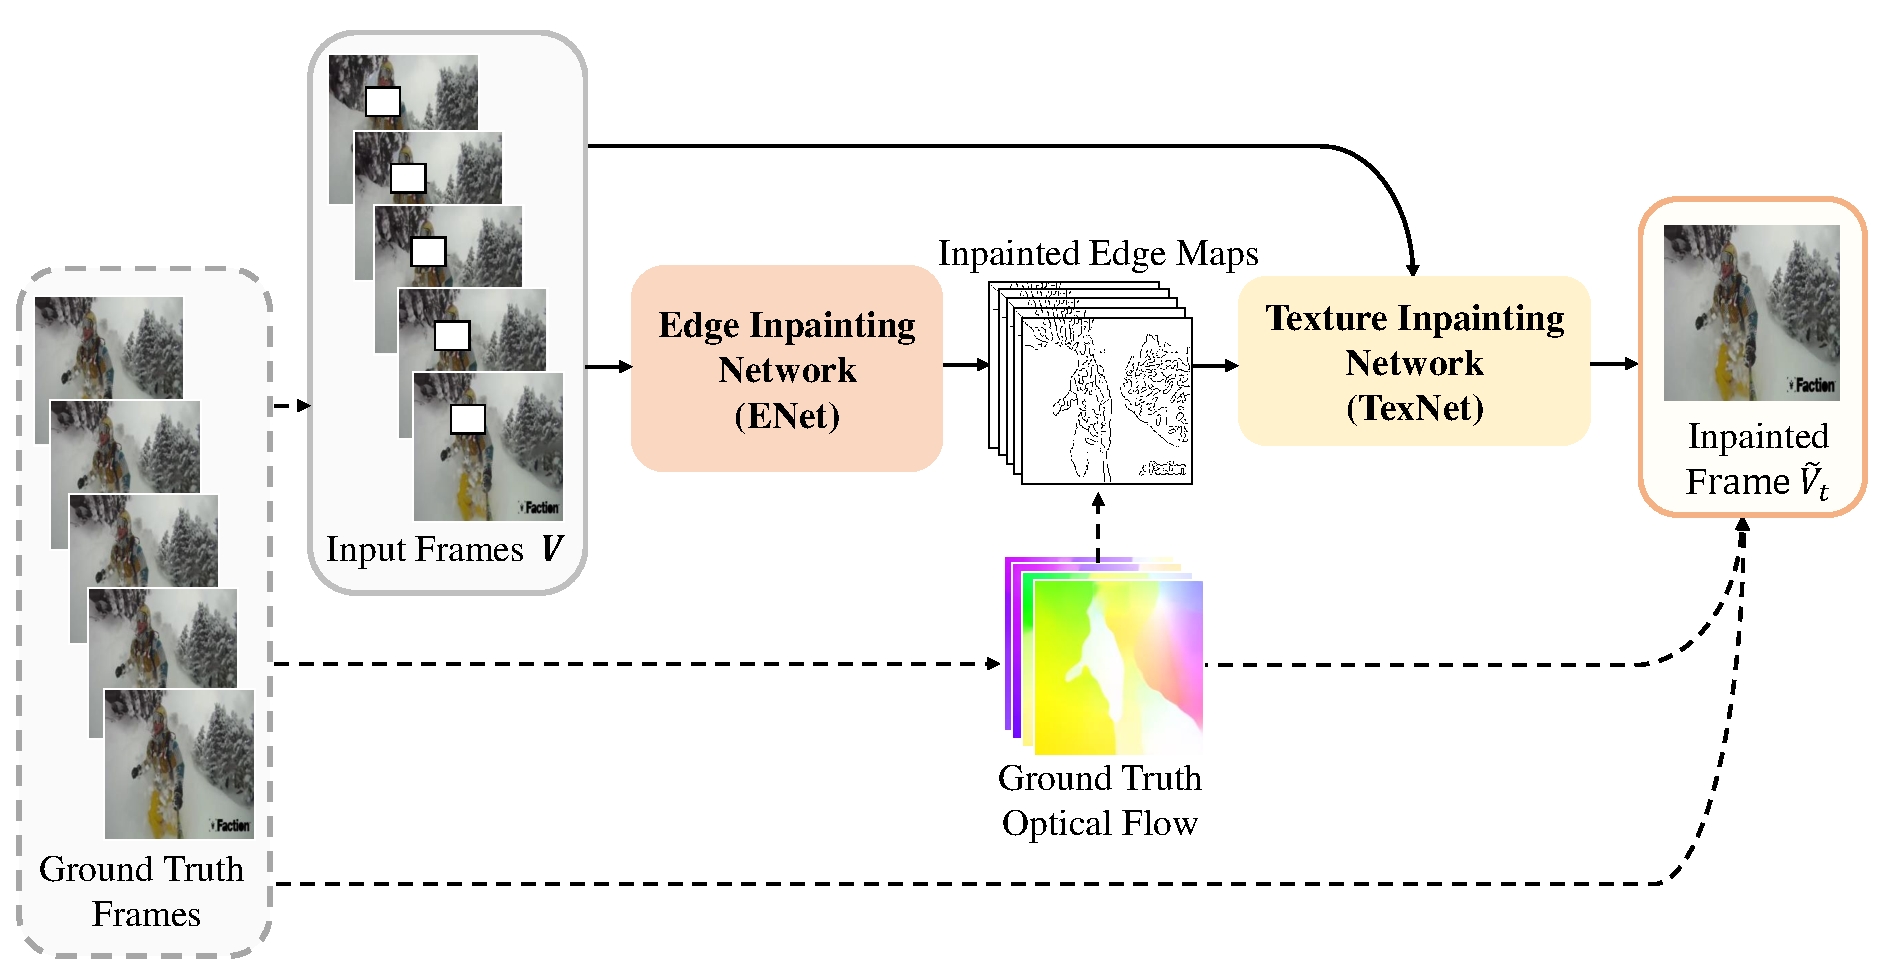
\includegraphics[width=1.01\columnwidth]{pipeline} 
	\caption{Overview of our structure-guided video inpainting network. We first complete the edges in the corrupted region by aggregating information from neighboring frames to represent the target structure using the ENet. Then, the TexNet synthesizes missing textures under the structural guidance of inpainted edges. Besides, the ground truth optical flow between frames is utilized during the training stage for both ENet and TexNet to enforce temporal coherence of completed contents, as illustrated by dotted lines.}
	\label{fig:overview}
\end{figure}






\section{Related Work}

%
\mdf{Image and video inpainting has been studied for decades. In this section, we mainly discuss four categories of related works, including (a) traditional methods of image inpainting, (b) patch-based video inpainting, (c) CNN-based image inpainting, and (d) deep video inpainting.  }


\paragraph{Traditional Image Inpainting Approaches}
Traditional methods of image and video inpainting can be divided into two categories, diffusion-based and patch-based methods. 
Diffusion-based methods \cite{bertalmio2000image,ballester2001filling,sridevi2019image} gradually propagate contents from surrounding areas to the missing region. 
%Li \emph{et al.}~\cite{li2016image} define diffusion coefficients according to the relation between the damaged pixels and neighborhood pixels.
%Li \emph{et al.}~\cite{li2017localization} attempt to solve the problem of localization of diffusion-based inpainted regions.
%Fractional-order nonlinear diffusion driven by difference curvature is proposed to produce clearer image details \cite{sridevi2019image}. 
However, this category of methods fails to handle large holes due to its assumption of local smoothness. 
%
Patch-based image inpainting methods, also called exemplar-based methods~\cite{bertalmio2003simultaneous,efros2001image,li2008patch,zhang2014image}, are more widely studied.
They formulate the completion task as a patch-based optimization problem. 
Barnes \emph{et al.}~\cite{barnes2009patchmatch} employ approximate nearest neighbor algorithm to fill the damaged regions.
Sangeetha \emph{et al.}~\cite{sangeetha2011combined} propose to propagate both linear structure and two-dimensional texture into the target region.
Ru{\v{z}}i{\'c} \emph{et al.} \cite{ruvzic2014context} introduce Markov random field to search the most matched candidates.
Ding \emph{et al.} \cite{ding_19nonlocal} employ nonlocal texture similarity and local intensity smoothness to produce natural-looking results.
Besides, some patch-based methods utilize low rank approximation. For example, Guo \emph{et al.} \cite{pb_lowrank2018} propose a simple two-stage low rank approximation to recover the corrupted region, which avoids time-consuming iterations.
Lu \emph{et al.} \cite{lu2018gradient} adopt gradient-based low rank approximation.
These patch-based methods fill the missing content by borrowing and aggregating the most similar patches based on low-level image features from known regions. However, they usually fail when there is insufficient information in known regions or image textures are too complicated.  
%

\paragraph{Patch-Based Video Inpainting} Patch-based methods are also widely studied for video inpainting \cite{wexler2007space,tcsvt2009,umeda2012removal,xu2015video}. 
They search similar patches and borrow appearances from known regions across neighboring frames to synthesize the unknown content. 
Wexler \emph{et al.} \cite{wexler2007space} constrain masked regions to synthesize coherent structures with respect to reference examples based on local structures. 
Umeda \emph{et al.} \cite{umeda2012removal} propose using directional median filter as complementation of patch-based filling.
Newson \emph{et al.} \cite{newson2014video} extend the 2D PatchMatch algorithm~\cite{barnes2009patchmatch} into 3D version to improve video inpainting quality.
Xu \emph{et al.} \cite{xu2015video} first complete motion field to guide the patch composition for video background completion.
Huang \emph{et al.} \cite{huang2016temporally} jointly estimate optical flow and textures to promote temporal coherence.
%
Another group of methods separate foreground and background apart, and then deal with the two parts with different algorithms, respectively.
%, naturally exists property difference between the.  
Ghanbari \emph{et al.} \cite{ghanbari2011contour} first separate foreground and background in videos, and fills the two parts accordingly with the help of contours.
Xia \emph{et al.} \cite{xia2011exemplar} make use of Gaussian mixture models to distinguish moving foreground and still background, and process them separately.   
%However, traditional metshods assume that there exist similar contents in known regions, thus fail to synthesize unseen appearances. 
However, in these patch-based video inpainting methods, the patch-searching process suffers from high computational complexity, thus limiting their usage in practical applications.



\begin{figure*}[!t]
	\centering
	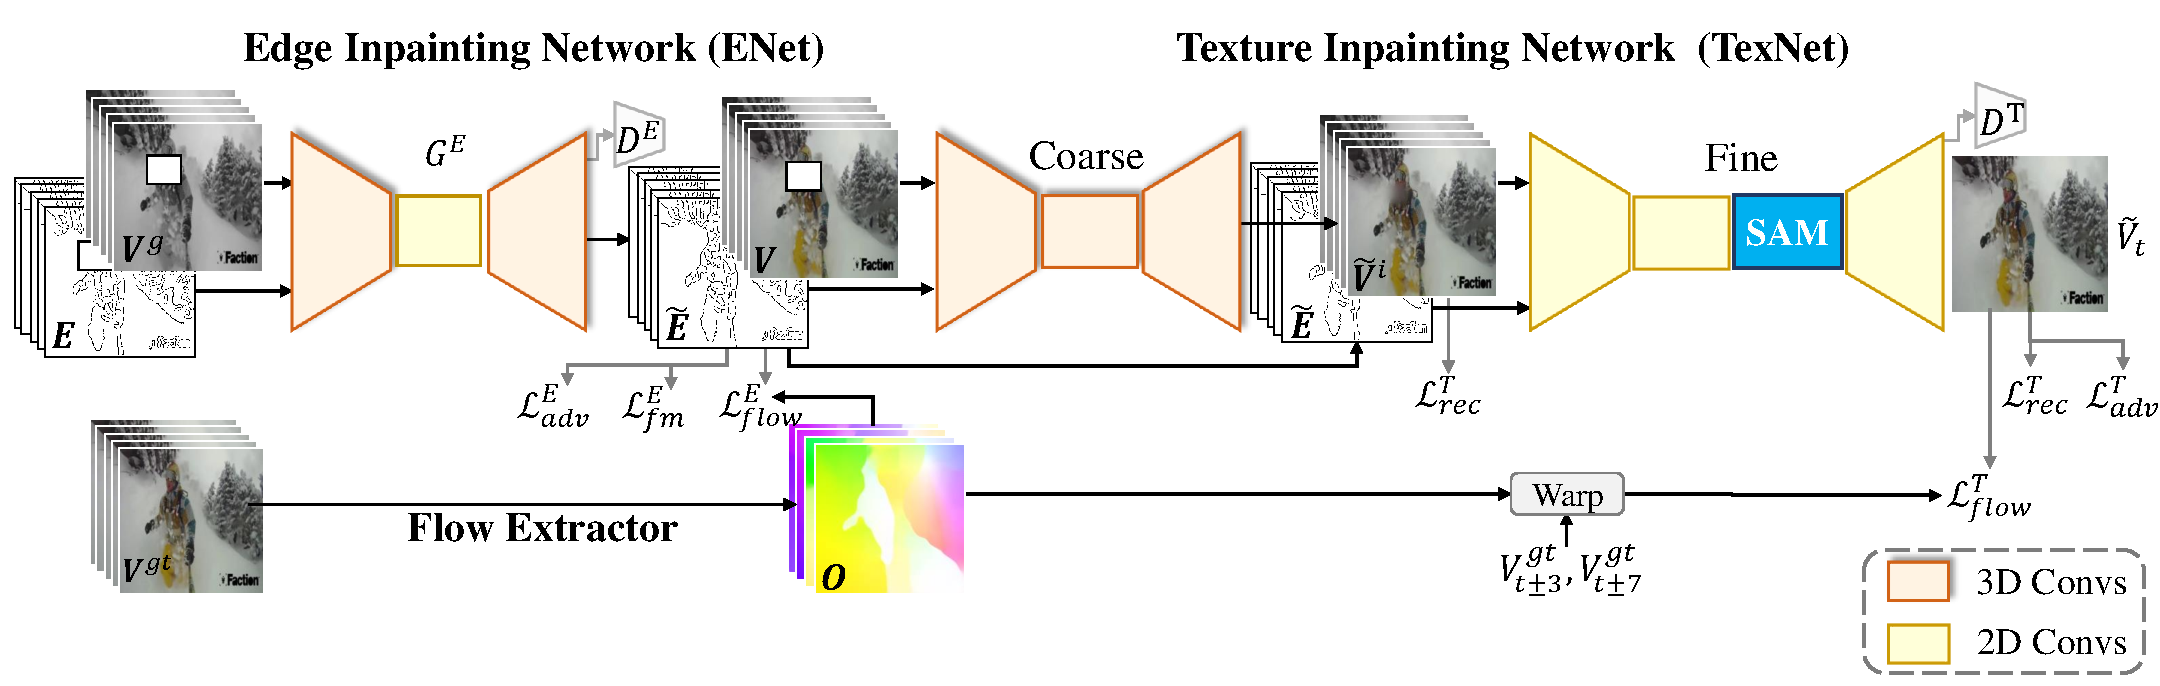
\includegraphics[width=2.05\columnwidth]{sti} % 
	\caption{The detailed architecture of our network. ENet adopts an encoder-decoder architecture to complete edges in the missing regions. TexNet utilizes a coarse-to-fine manner to inpaint the final frames. Ground truth optical flow between adjacent frames is employed in edge consistency loss and frame warping loss to enforce temporal coherence. }
	\label{fig:stiNet}
\end{figure*}

\paragraph{CNN-based Image Inpainting}
Recently, deep learning methods have achieved tremendous progress in the field
of computer vision. The tasks of image and video inpainting also have witnessed great promotion thanks to the capability of deep neural networks to capture high-level semantic information in images and videos.
%
A convolution neural network (CNN) is first introduced to directly synthesize image contents in the masked regions for image denoising and inpainting in \cite{xie2012image}.
To improve the photorealism of the synthesized content, a generative adversarial network is employed \cite{pathak2016context}. 
Then, Yang \emph{et al.} \cite{yang2017high} take advantages of multi-scale representation to boost details generation.
%by jointly training a generator and a discriminator in a minimax manner. 
Multiple discriminators are used to constrain both global and local coherence of image contents \cite{iizuka2017globally}.  
Yu \emph{et al.} \cite{yu2018generative} propose a contextual attention module in capturing long-range information.
Subsequent approaches solve more specific problems in image inpainting, for example, inpainting irregular holes with partial convolution~\cite{liu2018partialinpainting} or employing gated convolution \cite{yu2018free} for dynamic feature selection. 
While these methods tend to generate over-smoothed and blurry results, a two-stage approach is proposed to hallucinate edges first and then fill image colors using the edges as a prior \cite{nazeri2019edgeconnect}. 
Similarly, Xiong \emph{et al.} \cite{Xiong_2019_CVPR} predict contours of foreground objects to guide the inpainting process of masked regions.
Though high-quality static images with reasonable structure can be generated using these edge-based methods, simply extending it from image inpainting to video inpainting by 3D convolutions inevitably fails because of no guarantee on the temporal coherence, especially on the high-frequency signals. 
Besides, these methods simply utilize edges and contours as one additional channel of the image inpainting network, without exploiting the mutual relationship between edges and textures. 
In comparison, we design a structure attention module to better explore the structural guidance in synthesizing textures. 


%%% video inpainting 
\paragraph{Deep Video Inpainting}
Several video inpainting methods based on deep neural networks have been proposed recently, to fully utilize useful complementary information in neighboring frames.
%
The first deep-learning-based video inpainting method is CombCN \cite{wang2019video}, which jointly learns temporal structure and spatial details via 3D convolutions.
%%\cite{Xu_2019_CVPR} proposes a stacked convolution network to predict missing motion field and regards video inpainting as a pixel propagation problem. 
%
To enforce temporal coherence, features from neighboring frames are collected and refined to synthesize the missing content with recurrent feedback \cite{Kim_2019_CVPR1,Kim_2019_CVPR}. 
\mdf{OPN \cite{oh2019onion} uses the non-local formulation to calculate the similarity between pixels in reference and target frames, and then copies the contents based on the similarity.
%The similarity is between video contents.
Similarly, Copy-and-Paste \cite{lee2019copy} copies matching contexts in aligned reference frames and pastes them to the corrupted region.
However, both OPN and Copy-and-Paste only consider the texture correlation between neighboring frames, while ignoring high-level structures.
In comparison, we explore the correlation between structures and textures to achieve high-quality inpainting results.}  
%
Instead of filling pixel colors directly using CNNs, a deep flow-guided inpainting network is proposed in \cite{Xu_2019_CVPR} to estimate optical flow first in the missing region and then propagate pixel colors based on the completed flow.
However, these existing methods usually suffer from blurs and structural cracks in the synthesized frames since it is non-trivial to maintain fine details and sharp edges simultaneously when predicting temporally coherent pixel colors. 
In comparison, we propose to explicitly complete the target structure using edges, which are efficient due to their sparsity. To utilize structural information more effectively, we also introduce a structure attention mechanism. 
Under the structural guidance, more visually pleasing results could be synthesized with plausible structure and fine details. 

 






























\section{Approach}\label{sec:approach}


Our goal is to recover the missing contents in a corrupted video, with consideration of fine details and temporal consistency.
To produce a completed frame $\widetilde{V}_t$ at time $t$, we take total $T$ ($T=5$) frames $\boldsymbol{V}=\msset{V}$, as input to our inpainting network in each data batch. 
The corrupted regions \mdf{in the $T$ frames are indicated by binary masks $\boldsymbol{M}=\msset{M}$} where $M_t(p)=1$ indicates that pixel $p$ is corrupted in frame $V_t$. 
%
 
The detailed architecture of our inpainting network is shown in 
Fig.~\ref{fig:stiNet}.
It consists of three main components. 
The first part is an edge inpainting network (ENet) for structure inference that recovers edges in the missing regions of the input frames.
The second part is a coarse-to-fine texture inpainting network (TexNet) that aims to complete the missing contents with visual details under the guidance of hallucinated edges.
The third part leverages the ground truth motion flow as auxiliary constraints to enforce temporal coherence of both the completed edge maps and textures at the training stage.
%The ground truth motion flow is employed to guarantee the consistency of edges and aggregate previously synthesized frames to refine the current frame.
%During the inference stage, only the edge-guided inpainting path is used to complete the target frame, which generates high-quality inpainted results with low time cost.



\subsection{Edge Inpainting Network}
\label{sec:edgenet}
 
The edge inpainting network (ENet) completes image edges in the missing regions to depict scene structures and object shapes.
\mdf{From $T$ neighboring corrupted frames $\boldsymbol{V}$ as well as the corresponding set of binary masks $\boldsymbol{M}$}, a Canny edge detector is first applied to extract the corresponding edge maps $\boldsymbol{E}$ in the uncorrupted regions. %Notably, the edges in the masked regions in $\boldsymbol{E}^{i}$ are missed. 
%Given the incompleted grayscale images $\boldsymbol{X}^{g}$ of input frame, a canny edge detector is first used to generate initial edge maps. 
The input of ENet is \mdf{the concatenation of} the incomplete grayscale version of $T$ frames $\boldsymbol{V}^{g}$, initial edge maps $\boldsymbol{E}$, and their corresponding masks $\boldsymbol{M}$.
%
As shown in Fig.~\ref{fig:stiNet}, our ENet, denoted by $G^E$, is composed of a three-layer 3D encoder, eight 2D residual blocks, and a three-layer 3D decoder. 
%{\color{blue}Detailed network architecture implementation is listed in Table~\ref{tab:enet-arch1}.}
The 3D encoder and decoder are designed to \mdf{capture temporal coherence, which takes large computation consumption. The intermediate 2D residual blocks are efficient in aggregating spatial contexts in large spatial receptive fields. Under a limited number of network parameters, we can adopt more 2D convolution layers, thereby obtaining larger spatial receptive fields compared to 3D convolutions.
This hybrid 2D and 3D convolution network achieves a good balance between spatial and temporal coherence.}
The inpainted $T$ edge maps 	$\boldsymbol{\widetilde{E}}=\msset{\widetilde{E}}$ are obtained by:
\begin{equation}
	\label{eq:edgenet}
	\boldsymbol{\widetilde{E}}=G^E(\boldsymbol{E},\boldsymbol{V}^{g},\boldsymbol{M}).
\end{equation}

\mdf{Without any auxiliary information, the edge inpainting network ENet can be trained adversarially by}:
%
\begin{equation}
	\label{eq:loss_e_}
	\min\limits_{G^E} \max \limits_{D^E} \big(\mathcal{L}^E_{adv}+\lambda_1 \mathcal{L}^E_{fm}\big),
\end{equation}
%
where the discriminator $D^E$ follows the $70\times 70$ PatchGAN architecture \cite{Isola_2017_CVPR}. 
$\mathcal{L}^E_{adv}$ and $\mathcal{L}^E_{fm}$ are the adversarial loss and feature matching loss respectively. 
$\lambda_1$ is a hyper-parameter to balance the two terms.
%
$\mathcal{L}^E_{adv}$ tends to make the inpainted edge maps follow the distribution of real edge maps by
\begin{equation} \label{eq:edge_adver}
	\begin{aligned} 
		\mathcal{L}^E_{adv}  =&\mathbb{E}_{({E}_t^{gt},{V}_t^{g})}\big[logD^E({E}_t^{gt},{V}_t^{g})\big]\\ 
		+&\mathbb{E}_{({\widetilde{E}_t},{V}_t^{g})}\big[log\big(1-D^E ( {\widetilde{E}_t},{V}_t^{g})\big)\big].
	\end{aligned}
\end{equation}
% 
$\mathcal{L}^E_{fm}$ evaluates the feature-level similarity between ground truth and predicted edge maps, which is defined by:
%Feature matching loss was first proposed in \cite{wang2018high} and has been widely used in recent GANs.
%The feature matching loss is defined as:
\begin{equation}
	\label{eq:edge_fm}
	\mathcal{L}^E_{fm}=\sum_{t=1}^T\sum_{k=1}^L{\frac{1}{N_k}\left\| D^E_k({E}_t^{gt},{V}_t^{g})- D^E_k({\widetilde{E}_t},{V}_t^{g})\right\|_1},
\end{equation}
where $D^E_k$ is the $k$-th layer in the $L$-layer $D^E$, and $N_k$ is the element number of the output of $D^E_k$.
\mdf{We use the feature similarity loss $\mathcal{L}^E_{fm}$ instead of L1 reconstruction loss because that L1 reconstruction loss is sensitive to small drifts and noises for sparse edge maps.}
%By considering both feature-level and image-level similarities in Eq.~\eqref{eq:loss_e_}, the edge generator $G^E$ can be trained to produce plausible and structurally rational edge maps.
%Note that the discriminator $D^E$ is not optimized by the feature matching loss term. It plays as a feature extractor to optimize the generator $G^E$ for producing plausible edge maps $\boldsymbol{E}$.
As a result, the proposed hybrid 3D and 2D convolution architecture and the adversarial loss enable our ENet to hallucinate the missing edges accurately and efficiently.
An example of the generated edge map is given in Fig.~\ref{fig:coarse-fine} (a) and (b). 
The stripe pattern on the dog is well inferred from neighboring frames. 


\begin{figure}[t]
	\centering
	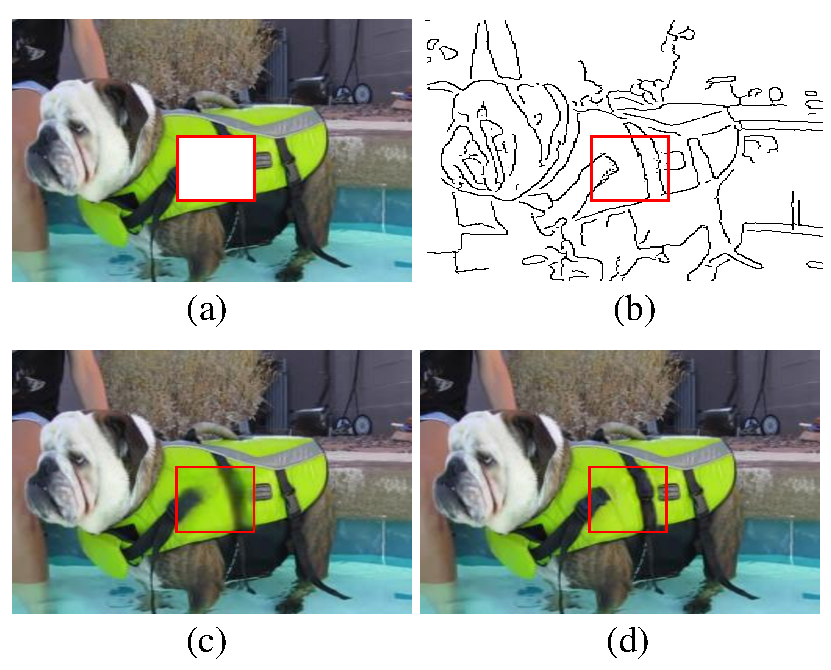
\includegraphics[width=0.8\columnwidth]{coars-fine} 
	\caption{To inpaint missing regions in a corrupted frame (a), our ENet first completes corresponding sparse edges (b), which well represent the structure of the missing contents. Then TexNet progressively replenishes textures under the guidance of synthesized edges from coarse (c) to fine (d).}
	
	\label{fig:coarse-fine}
\end{figure}




\begin{figure}[t]
	\centering
	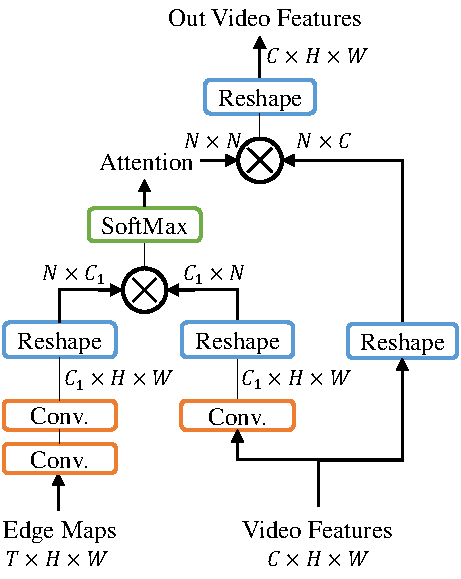
\includegraphics[width=0.65\columnwidth]{SAM}
	\caption{Architecture of the structure attention module. $C$ is number of channels of the input video features, and $N=H\times W$. $\otimes$ represents matrix multiplication. Usually, we set $C_1=C/8$.}
	\label{SEM}
\end{figure} 





\subsection{Edge-Guided Texture Inpainting Network}

 
With the $T$ completed edge maps $\boldsymbol{\widetilde{E}}$ for the $T$ neighboring frames $\boldsymbol{V}$, we then fill the image texture using TexNet.
Notably, the image structure,~\emph{e.g.,} object shapes, is well represented by the completed edge maps $\boldsymbol{\widetilde{E}}$.
Thus, it becomes easier to fill the missing texture with the structural guidance of $\boldsymbol{\widetilde{E}}$.
%
To synthesize realistic frame textures, our TexNet adopts a coarse-to-fine architecture, as shown in Fig.~\ref{fig:stiNet}.
Specifically, TexNet {\color{blue}$G^T$} consists of a coarse inpainting network {\color{blue}$G_c^T$} and a refinement network {\color{blue}$G_r^T$}.
%
%The input of TexNet is the concatenation of  $\boldsymbol{\widetilde{E}}$, $\boldsymbol{V}$, and $\boldsymbol{M}$.
First, the coarse inpainting network consists of a set of 3D convolutions to capture the spatio-temporal contexts from the hallucinated edge maps and the corrupted input frames, and produces a rough completion $\boldsymbol{\widetilde{V}}^i$ for the $T$ frames with colors and textures. {\color{blue}The input of $G^T_c$ is the concatenation of $T$ frames $\boldsymbol{V}$, the synthesized edge maps $\boldsymbol{\widetilde{E}}$, and the masks $\boldsymbol{M}$ to produce $T$ rough inpainting frames:}
{\color{blue}
	\begin{equation}
	\begin{aligned}
	\label{eq:coarsenet}
	\boldsymbol{\widetilde{V}}^i=G_{c}^T(\boldsymbol{V},\boldsymbol{\widetilde{E}},\boldsymbol{M}).
	\end{aligned}
	\end{equation}
}
%The 3D coarse network incorporates neighboring frames by convolutions of the time dimension.
Then, the refinement network takes {\color{blue}the concatenation of} the rough inpainting results $\boldsymbol{\widetilde{V}}^i$, the synthesized edge maps $\boldsymbol{\widetilde{E}}$, and the masks $\boldsymbol{M}$ as inputs to further refine texture details in $\boldsymbol{\widetilde{V}}^i$ with the structural guidance of edges $\boldsymbol{\widetilde{E}}$. 
Notably, only 2D convolutional layers are used in the refinement network to improve inference efficiency. 
%For the corrupted region, our ENet first completes sparse edges which well represent the structure of the missing content, then TexNet progressively replenishes textures under the guidance of synthesized edges.
{\color{blue}
	The refinement network finally reconstructs current frame:
	\begin{equation}
	\label{eq:refinenet}
	\widetilde{V}_t=G_{r}^T(\boldsymbol{\widetilde{V}}^i,\boldsymbol{\widetilde{E}},\boldsymbol{M}).	
	\end{equation}
}
Besides of taking $\boldsymbol{\widetilde{E}}$ as an auxiliary input in the refinement network, we further design a structure attention module (SAM) to fully encode the structural information.
The detailed implementation of SAM is given in Fig.~\ref{SEM}.
\mdf{The input of SAM consists of the intermediate video features extracted from the rough inpainting frames $\boldsymbol{\widetilde{V}}^i$ and the edge maps $\boldsymbol{\widetilde{E}}$.} 
First, the intermediate video features and embedded edge features are interacted to calculate the latent structure-texture correlation via matrix multiplication. 
After a SoftMax operation, the normalized attention map is obtained while it conveys the correlation between sparse structures and video features.
%
The normalized attention map is applied to the intermediate video features, and the structure information is thus embedded in TexNet, which can better extract useful structural information from edges.
{\color{blue}
The main difference between our SAM and self attention module \cite{vaswani2017attention} is that self attention only considers texture correlation, while our SAM focuses on edge-texture correlation to overcome the over-blurry problem in video inpainting.}
By introducing structural guidance in the refinement network, the inpainted content by TexNet becomes more realistic, as Fig.~\ref{fig:coarse-fine} (d) shows.

%The core insight of SAM is to explicitly capture the spatial correlation between edges and textures, which is regarded as a guidance in the texture generation processing.

%Fig.~\ref{fig:coarse-fine} shows an example of our structure-guided inpainting result. 

The coarse inpainting network and the refinement network in TexNet are trained end-to-end in an adversarial manner by:
%
\begin{equation}
	\label{eq:1}
	\min\limits_{G^T} \max \limits_{D^T} \big(\mathcal{L}^{T}_{rec}+\mathcal{L}^T_{adv}\big),
\end{equation}
\mdf{where the discriminator $D^T$ follows the same architecture as $D^E$.}
%
Inspired by \cite{nazeri2019edgeconnect}, the first term $\mathcal{L}^{T}_{rec}$ is the $l_1$-reconstruction loss to measure the difference between predicted video frames and the ground truth video frames $\boldsymbol{V}^{gt}$.
Differently, we penalize both \mdf{the single refined frame $\widetilde{V}_t$ and the coarse predictions of $T$ frames $\boldsymbol{\widetilde{V}}^i$} by:
\begin{equation}
		\label{eq:loss_rec}
	\begin{aligned}
		\mathcal{L}^{T}_{rec}&=\frac{1}{\left\|M_t \right\|_1}\left\|(\widetilde{V}_t-V^{gt}_t)\odot M_t\right\|_1,\\ 
		&+\lambda_2*\frac{1}{\left\|\boldsymbol{M} \right\|_1}\left\|(\boldsymbol{\widetilde{V}}^i-\boldsymbol{V}^{gt})\odot \boldsymbol{M}\right\|_1,
	\end{aligned}
\end{equation}
where $V^{gt}_t$ denotes the ground truth frame of time $t$, and $M_t$ is the corresponding binary mask. 
%
The extra adversarial loss $\mathcal{L}^T_{adv}$ is introduced in Eq.~\eqref{eq:1} to promote the visual realism of the generated frame $\widetilde{V}_t$ by:
	%$\mathcal{L}^I_{adv}$ is defined as:
	\begin{equation}
		\label{eq:inp_adver}
		\mathcal{L}^T_{adv}=\mathbb{E}[logD^T(V^{gt}_t)]+\mathbb{E}[log\big(1-D^T(\widetilde{V}_t)\big)].
	\end{equation}
%$\mathcal{L}^T_{adv}$ enforces the generated frame to be more realistic.


The coarse and refinement networks can be effectively trained jointly with the combined loss of $\mathcal{L}^T_{rec}$ and $\mathcal{L}^T_{adv}$.
The results in Fig.~\ref{fig:coarse-fine} (c) and (d) show that the coarse network completes the missing content with rough textures under the structure guidance of inpainted edges and the refinement network exactly refines the inpainting results with more sharp contours and realistic textures.

% enables the TexNet to first give a coarse inpainting results, and then refine the results with the structure guidance.
%It can be seen that the coarse-to-fine architecture


 

\subsection{Flow-Guided Temporal Coherence Enhancement}
\label{sec:fec}
Besides the structural guidance, motion information is also considered in our method to enhance temporal consistency among the recovered frames.
We employ optical flows in the training stage of both ENet and TexNet \mdf{using self-supervision of neighboring frames.}
A set of flow maps \(\boldsymbol{O}\) between the current frame $V_t^{gt}$ and its neighboring frames are generated using a pre-trained flow extraction network, such as FlowNet2.0~\cite{Flownet_2017_CVPR}.
Specifically, \(\boldsymbol{O}\) consists of four flow maps \((O_{t\Rightarrow t-7}, O_{t\Rightarrow t-3}, O_{t\Rightarrow t+3}, O_{t\Rightarrow t+7})\).
 
 
In terms of the ENet which completes the missing edges, \(\boldsymbol{O}\) is used to first warp the neighboring edge maps to the current frame, and then compute the consistency between neighboring edge maps.  
A flow-guided edge consistency loss is defined as:
%
\begin{equation}
	\label{eq:flow_edge}
	\mathcal{L}^E_{flow}=\sum_{k}\frac{1}{\left\|M_{t} \right\|_1}\left\|\Big(\widetilde{E}_{t}-\phi\big(O_{t\Rightarrow t+k},E_{t+k}^{gt}\big)\Big)\odot M_{t}\right\|_1,
\end{equation}
where $\phi\big(O_{t\Rightarrow t+k},E_{t+k}^{gt}\big)$ is the warping operation which warps a neighboring edge map $E_{t+k}^{gt}$ to the target frame according to the estimated optical flow $O_{t\Rightarrow t+k}$.
$k$ denotes the index of neighboring frames ($k\in \left\{-7,-3,+3,+7 \right\}$). 
\mdf{By introducing this additional flow-guided edge consistency loss $\mathcal{L}^E_{flow}$ when training ENet, the original loss function (Eq.~\eqref{eq:loss_e_}) becomes:}
\begin{equation}
\label{eq:loss_e}
\min\limits_{G^E} \max \limits_{D^E} \big(\mathcal{L}^E_{adv}+\lambda_1 * \mathcal{L}^E_{fm}+\mathcal{L}^E_{flow}\big).
\end{equation}

 

\mdf{Similarly, when we train the TexNet, we further enforce the temporal coherence of synthesized neighboring frames via a flow-guided texture consistency $\mathcal{L}^T_{flow}$ by:} 
\begin{equation}
	\label{eq:inp_flow}
		\mathcal{L}^T_{flow}=\sum_{k}\frac{1}{\left\|M_{t} \right\|_1}\left\|\Big(\widetilde{V}_{t}-\phi\big(O_{t\Rightarrow t+k},V_{t+k}^{gt}\big)\Big)\odot M_{t}\right\|_1,
	\end{equation}
where $k \in \{-7,-3, 3, 7\}$, and $\phi\big(O_{t\Rightarrow t+k},V_{t+k}^{gt}\big)$ warps the neighboring frame $V_{t+k}^{gt}$ to the target frame using the estimated flow $O_{t\Rightarrow t+k}$. 
\mdf{The flow warping loss $\mathcal{L}^T_{flow}$ is added to the objective function of TexNet, which converts Eq.~\eqref{eq:1}
to:}
\begin{equation}
\label{eq:1_}
\min\limits_{G^T} \max \limits_{D^T} \big(\mathcal{L}^{T}_{rec}+\mathcal{L}^T_{adv} +\mathcal{L}^T_{flow}\big).
\end{equation}

After adding the motion guidance to both the training processes of ENet and TexNet, the temporal consistency can be enhanced in both edge generation and texture inpainting.
Since the motion is only used in the training stage, the inference of the proposed structure-guided inpainting method is efficient and effective.
 






	

\section{Experiments}\label{sec:exp}
To evaluate the effectiveness of our approach, we conduct a series of comparison experiments and ablation studies on two widely used datasets,~\emph{i.e.,} YouTubeVOS \cite{xu2018Youtube} and DAVIS \cite{davis_2017}, under different settings.
%We test on two datasets, YouTubeVOS \cite{xu2018youtube} and DAVIS \cite{davis_2017}, to compare the proposed STSENet with state-of-the-art methods. %Several ablation studies are conducted to prove the effectiveness of spatial details and temporal information in video inpainting.

\subsection{Experimental Settings}
\noindent \textbf{Mask Setting.} Considering different real-world applications, we test four kinds of mask settings in this paper, which are different in shapes and positions of the missing regions. 
%The first and the second settings aims to recover rectangular regions, which are common in watermark removal.
\begin{enumerate}
\item Fixed square mask: The size and position of the missing square regions are fixed through the whole video. 
\item Moving square mask: The position and size of the square masks change over frames. 
\item Free-from mask: We apply irregular masks which imitate hand-drawn masks on each frame, following \cite{liu2018partialinpainting}. 
\item Foreground object mask: This type of mask is defined to line out foreground objects in videos and used for testing object removal.
\end{enumerate}

\noindent\textbf{Dataset.} 
YouTubeVOS and DAVIS are widely used for evaluating video inpainting results in recent studies.
YouTubeVOS consists of 4,453 video clips that contain more than 70 categories of common objects. 
The videos are split into three parts, 3,471 for training, 474 for validation, and 508 for testing. Since YoutubeVOS has no dense foreground mask annotations, we only use it for evaluation under mask settings (1), (2), and (3). 
% 
DAVIS dataset contains 90 video sequences that are annotated with foreground object masks for test and 60 unlabeled videos for training.


\begin{figure*}[tb]
	\centering
	\includegraphics[width=\textwidth]{viszong} % Reduce the figure size so that it is slightly narrower than the column. Don't use precise values for figure width.This setup will avoid overfull boxes. 
	\caption{Comparison with state-of-the-art methods on the YouTubeVOS dataset under different mask settings. Our method produces results with more complete object structures and finer details. %\cxj{Modify reference number at last.} 
	}
	\label{viszong}
\end{figure*}



\begin{table*}[t]
	\caption{Comparisons with four state-of-the-art methods on YouTubeVOS. Our method outperforms all other methods on three metrics, with fast inference speed.}\smallskip
	
	\centering
	\resizebox{2.0\columnwidth}{!}{
		\smallskip\begin{tabular}{c|c|c|c|c|c|c|c|c|c|c }
			\hline
			&\multicolumn{3}{c|}{Fixed Square Mask}& \multicolumn{3}{c|}{Moving Square Mask}&\multicolumn{3}{c|}{Free-Form Mask}&Inference \\
			\cline{2-10} 
			&PSNR & SSIM & FID & PSNR & SSIM & FID & PSNR & SSIM & FID&Speed (fps)\\
			\hline
			Edge-Connect \cite{nazeri2019edgeconnect} &28.6446 &0.9484  &   38.2116  &    
			30.7478 & 0.9647 &  16.2739  &
			25.6693  & 0.9088 &  43.0366&22.81 \\
			\hline
			CombCN \cite{wang2019video} &27.9668 & 0.9515 &  40.7199  &     
			31.5776    & 0.9678 &  13.8383&   
			32.1862 & 0.9626 & 19.1191 &8.1634 \\
			\hline
			
			
			DVI \cite{Kim_2019_CVPR1}& 28.0846&0.9468 &  39.9377  & 
			36.8598    & 0.9728 &7.2315  &
			33.5549    & 0.9646 & 9.3797&1.2275  \\
			\hline
			DFVI \cite{Xu_2019_CVPR} &29.0531 & 0.9497 &  32.8860  & 
			37.8241& 0.9772 &6.3746  &
			32.6287 &0.9618  &  11.1501&0.5620 \\
			\hline
			
			\hline
			
			
			
			Ours &\textbf{30.0590} &\textbf{0.9543}&   \textbf{27.2431} &
			\textbf{38.8186} & \textbf{0.9824} & \textbf{2.3455} &
			\textbf{35.9613}  & \textbf{0.9721}&  \textbf{ 5.8694} &5.1546\\
			
			\hline
			
			
		\end{tabular}
	}
	\label{tab:sem}
\end{table*}





\noindent \textbf{Implementation details and Evaluation Metrics.} 
All the models are tested on a TITAN X (Pascal) GPU with frame size $256 \times 256$.
For training data, we randomly sample a training clip every 40 frames from each video in the dataset. Our training process consists of three steps. First, we train ENet with learning rate set as $1e-4$ for $G^E$ and $1e-5$ for $D^E$. 
Then we train TexNet while fixing ENet. The learning rate is set as $1e-4$ for $G^T$, and $4e-4$ for $D^T$.
We first train ENet and TexNet without flow-constrained losses, and then add the flow losses to finetune the networks.
%ensemble module is finally trained while fixing all the other modules. Learning rate is $1e-4$.
An Adam optimizer with $\beta=(0.9, 0.999)$ is used for all sub-network training.
%We do not use weight decay.
As for the hyper-parameters, we set $\lambda_1=10.0,\lambda_2=0.2$.
%, \lambda_3=0.1$.

Different data preparations and evaluation metrics are used according to mask settings. We randomly generate masks for training videos in terms of mask settings (1), (2), and (3). 
Masked videos are used for testing.
Three commonly-used metrics, including structural similarity index (SSIM) \cite{wang2004image}, peak signal-to-noise ratio (PSNR), and Fr{\'e}chet Inception Distance (FID) \cite{heusel2017gans} are used to quantitatively evaluate the performance of our method. 
For the mask setting (4), for each training video, we randomly select a test video from the 90 test videos in the DAVIS dataset and apply its masks for the current training video with random rotation, scaling, and translation.
Our inpainting network is first trained on the YoutubeVOS dataset and then finetuned on the DAVIS dataset. 
Since there are no ground truth videos available for this mask setting, we can not conduct quantitative evaluations to measure the output quality. In contrast, a user study is conducted for video foreground object removal.  


 


\subsection{Evaluation of Video Inpainting on YouTubeVOS}
We compare the proposed method with four state-of-the-art video inpainting methods \cite{nazeri2019edgeconnect,wang2019video,Kim_2019_CVPR1,Xu_2019_CVPR}
for the first three mask settings on the YouTubeVOS dataset.
%
We train \cite{nazeri2019edgeconnect,Xu_2019_CVPR} using their published codes and re-implement \cite{wang2019video} according to their paper. As for \cite{Kim_2019_CVPR1}, we use the officially provided model.

The quantitative results and inference speeds are reported in Table~\ref{tab:sem}.
It shows that our method outperforms state-of-the-art methods on the three metrics, demonstrating the effectiveness of introducing structure guidance into video inpainting.
Moreover, our method is also very efficient, e.g., four times faster than DVI \cite{Kim_2019_CVPR1} and nine times faster than DFVI \cite{Xu_2019_CVPR}. 
%We also notice that the best performance is typically obtained when using moving square masks for each individual approach. It indicates that these inpainting network can learn complementary information from neighboring frames.
Some inpainting examples are shown in Fig.~\ref{viszong}.
Compared with existing methods, the inpainting results predicted by our method are more realistic with finer details. 
We can observe that the frames completed using our method contain sharper object boundaries. This is achieved by the effectiveness of structure information in video inpainting.
%
It can also be seen that our method produces temporally smooth results when observing neighboring frames. 
%\cxj{show results?}


Compared with the 2D image inpainting method Edge-Connect\cite{nazeri2019edgeconnect},
which also predicts edges to represent the target structure,
our method greatly increases the completion performance by leveraging neighboring frames to complete edges and synthesize textures. 
Thus, our method can generate more temporally coherent and realistic contents. The inference speed of Edge-Connect is faster than our method since it does not consider axillary temporal information between frames. 
%
Compared with the second-best video inpainting method DFVI \cite{Xu_2019_CVPR}, our method produces frames with finer structural details. Besides, only ENet and TexNet are used to directly predict final outputs in the testing period in our method, while DFVI requires iterative pixel propagation. Thus the inference speed of our method is much faster than that of DFVI.
%
%% Time performance analysis 
Both the quantitative and qualitative results demonstrate that our method is not a naive extension to utilize structure information in video inpainting.
The well designed network architecture fully exploits structural guidance in video inpainting and brings large performance gain.




\begin{figure}[!t]
	\centering
	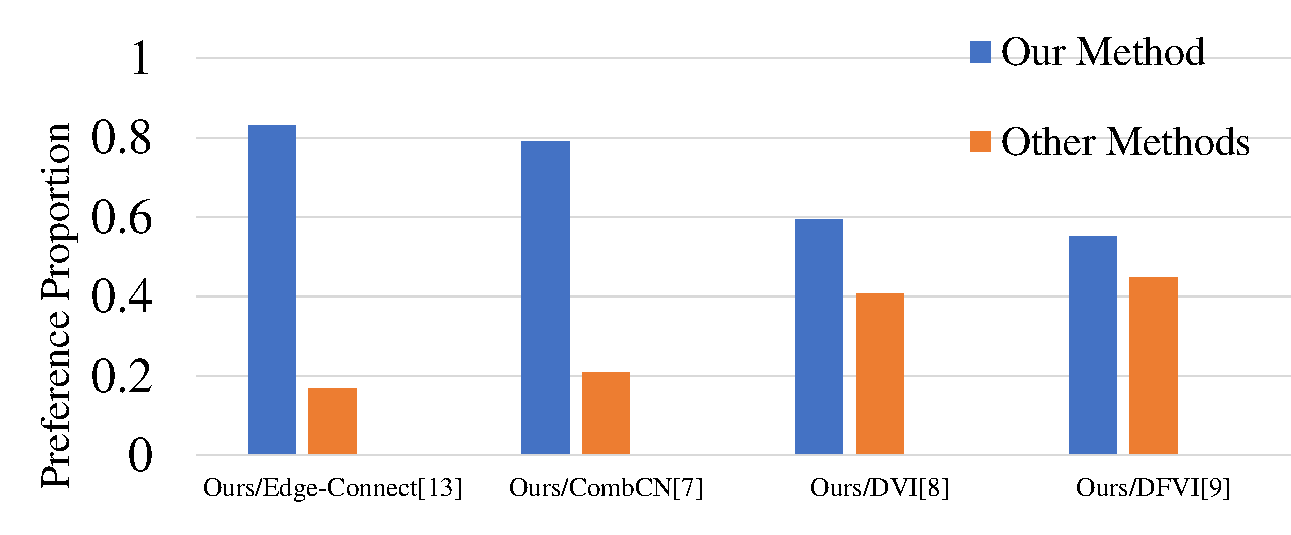
\includegraphics[width=1.0\columnwidth]{userstudy} % Reduce the figure size so that it is slightly narrower than the column. Don't use precise values for figure width.This setup will avoid overfull boxes. 
	\caption{Results of user study. The restored videos using our method are preferred by more participants compared with other state-of-the-art methods. }
	\label{userstudy}
\end{figure}



\begin{figure}[!t]
	\centering
	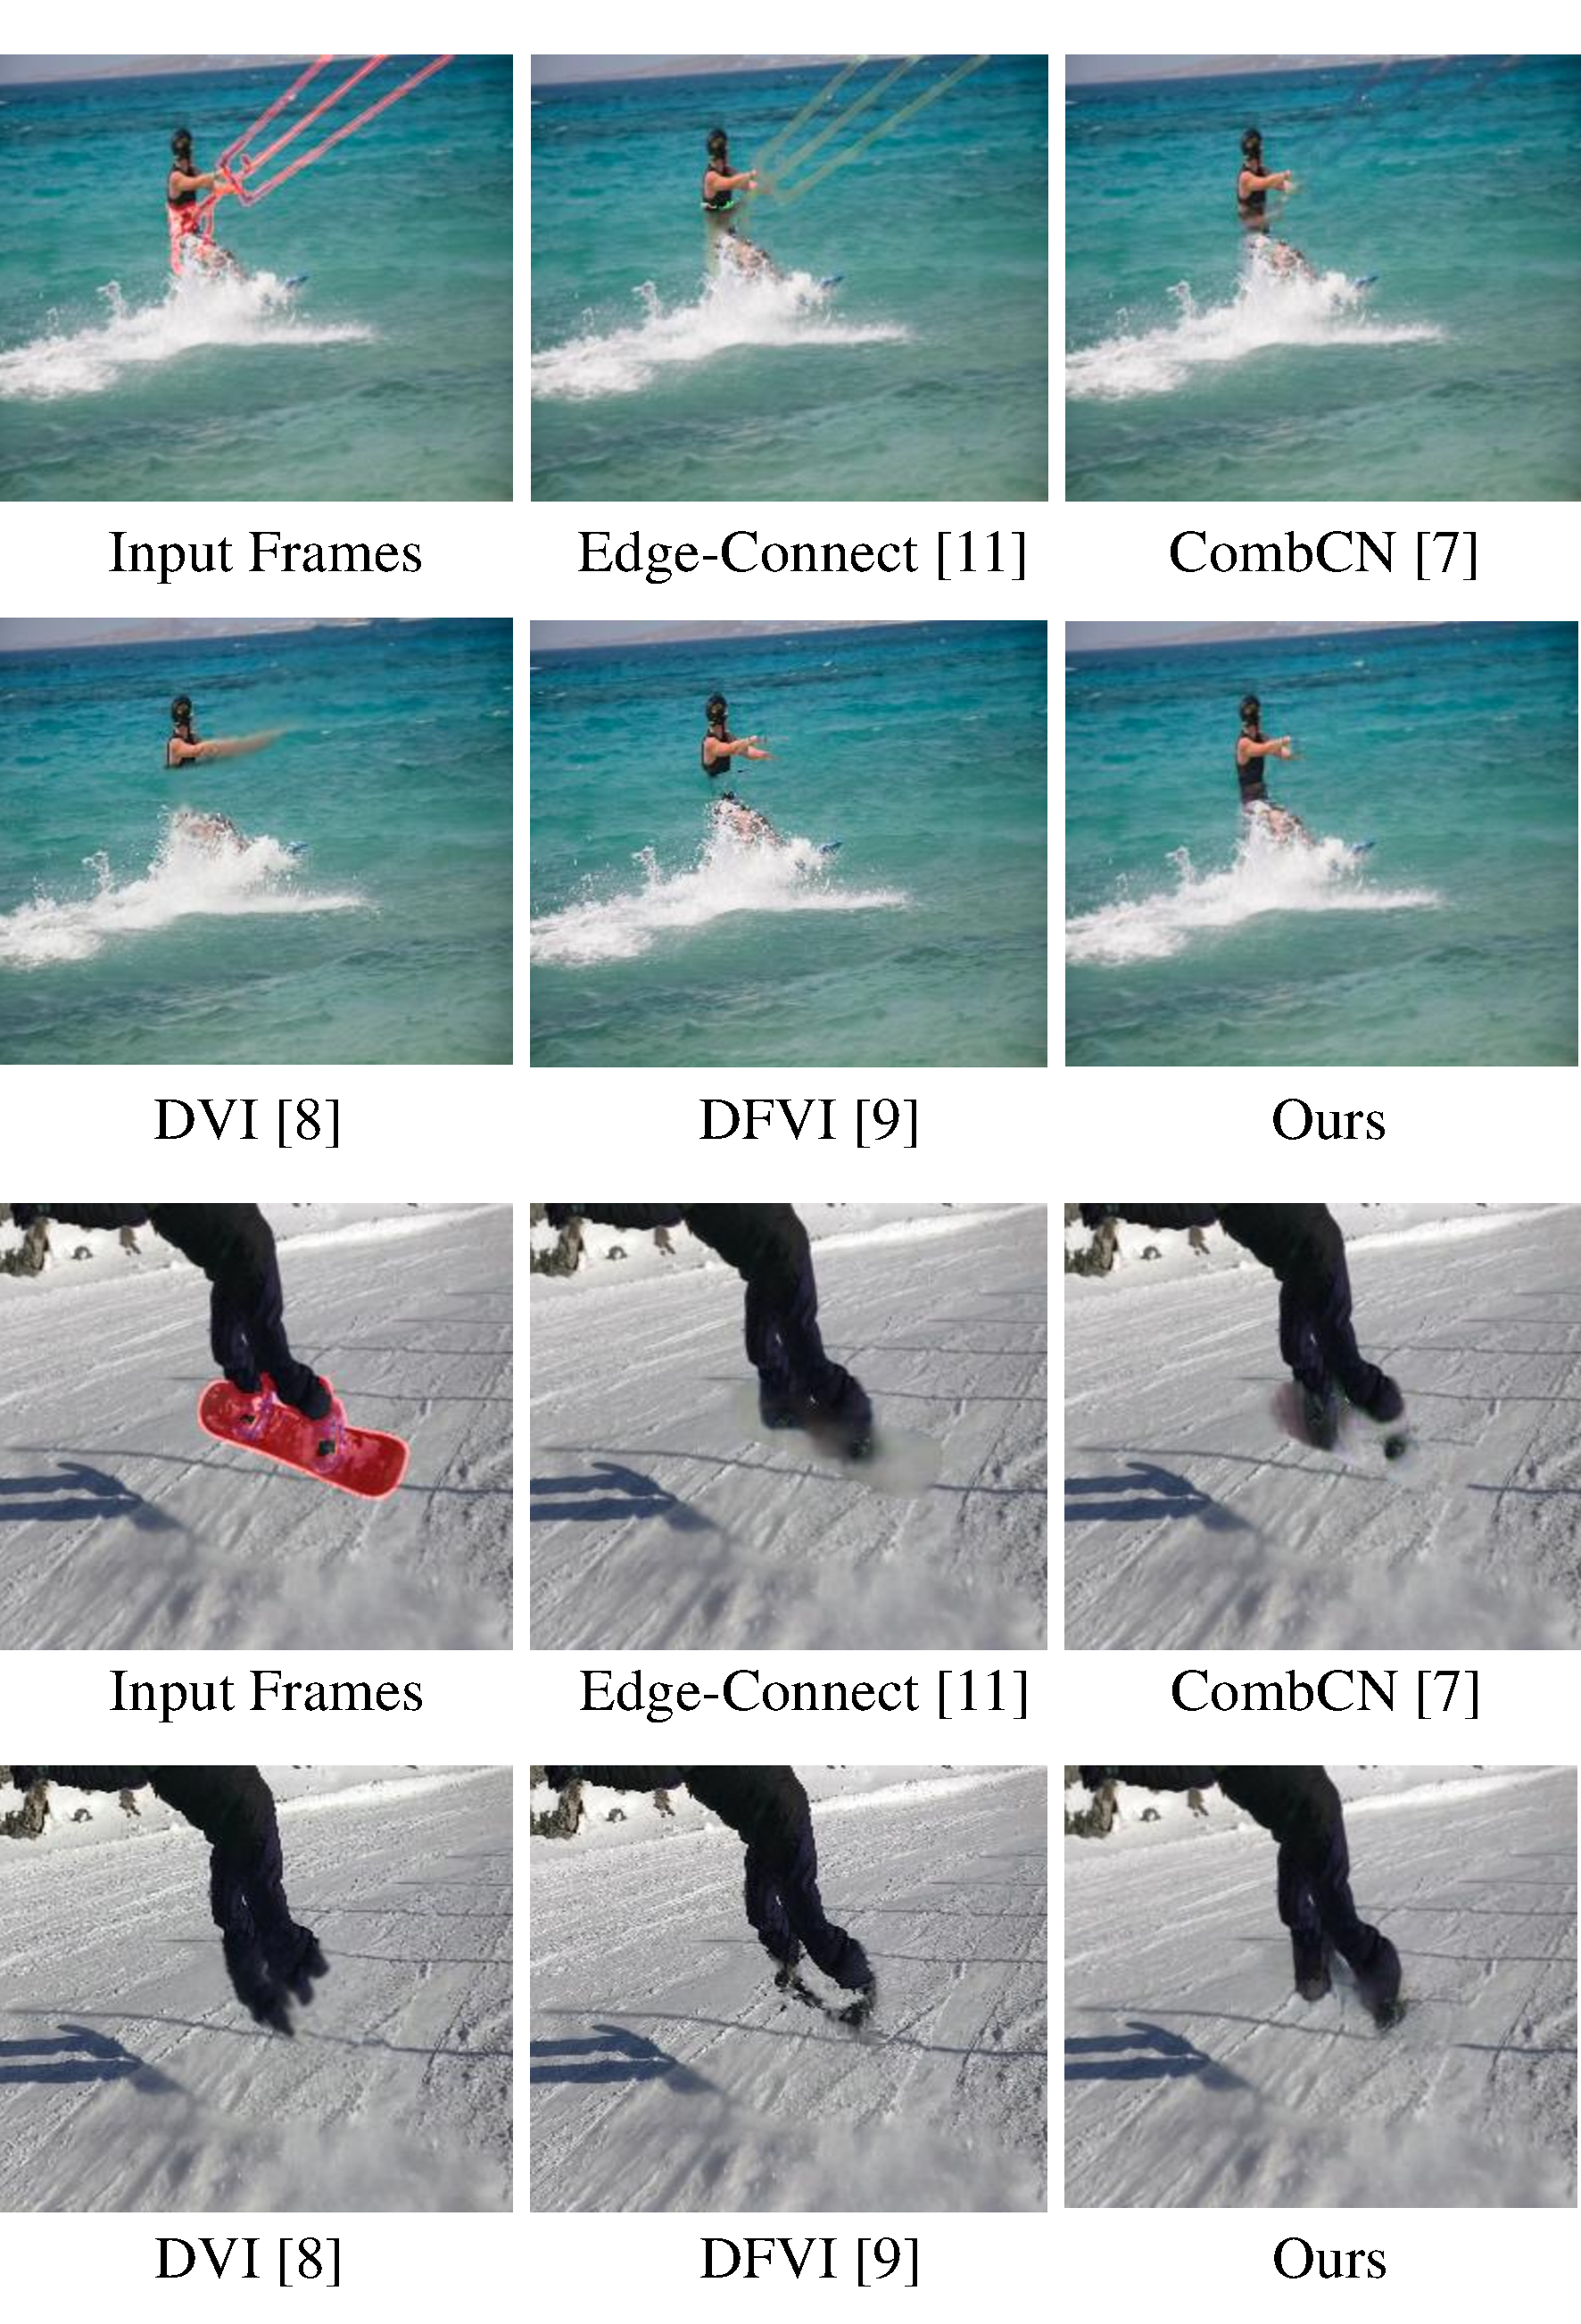
\includegraphics[width=0.85\columnwidth]{vis_forg} % Reduce the figure size so that it is slightly narrower than the column. Don't use precise values for figure width. This setup will avoid overfull boxes. 
	\caption{Results of object foreground removal. The red masks in input frames indicate the objects to be removed. Our method produces results with plausible structures and details.}
	\label{vis_forg}
\end{figure}


\subsection{Object Removal on DAVIS}


In regard to the foreground object mask setting that aims to remove undesired objects in videos, there is no ground truth for quantitative evaluation. 
Therefore, we conduct a user study on the DAVIS dataset to evaluate the visual quality of our method, compared with the four methods \cite{nazeri2019edgeconnect,wang2019video,Kim_2019_CVPR1,Xu_2019_CVPR}.
%
In each test, we show three videos to the subject at the same time. The original video with red masks indicating objects to remove is shown in the middle, while the inpainting results of our method and one of the other four methods are shown on the two sides in random order.
%  
The subjects can watch the videos repeatedly to better evaluate the differences.
For each video triplet, the subject is asked to choose which inpainting video is preferred.
44 subjects participated in our user study. 
Each participant watched averagely 20 triplets. 
Therefore, each pair of methods is compared about 220 times.
%Each method is compared about 200 times.

%


\begin{table*}[!t]
	\caption{Ablation studies on YouTubeVOS. Structure inference, structure attention model, and flow constrained loss are demonstrated effective in video inpainting.}\smallskip
	
	\centering
	\resizebox{1.8\columnwidth}{!}{
		\smallskip\begin{tabular}{c|c|c|c|c|c|c|c|c|c|c }
			\hline
			&\multicolumn{3}{c|}{Fixed Square Mask}& \multicolumn{3}{c|}{Moving Square Mask}&\multicolumn{3}{c|}{Free-Form Mask}&Inference \\
			\cline{2-10} 
			&PSNR & SSIM & FID & PSNR & SSIM & FID & PSNR & SSIM & FID&Speed (fps)\\
			
			\hline
			
			
			TexNet &28.0174 &0.9494  &  42.7164   &    
			33.8131 &  0.9705  &8.2390    & 
			30.0680& 0.9390 & 20.6358&7.6335
			\\
			\hline
			+Edge  &29.5242 &  0.9520& 36.2097   &    
			37.6630    & 0.9798 &3.5161    &    
			33.8206    &0.9659  &    6.6651& 5.2356 \\
			\hline
			
			+SAM &29.9918 &  0.9533 &  27.4198  &    
			38.2433    & 0.9807 &   2.5083  &    
			35.7783    &0.9712  &   5.8786 & 5.1546\\
			\hline
			
			
			
			
			+Flow &\textbf{30.0590} &\textbf{0.9543}&   \textbf{27.2431} &
			\textbf{38.8186} & \textbf{0.9824} & \textbf{2.3455} &
			\textbf{35.9613}  & \textbf{0.9721}&  \textbf{ 5.8694} &5.1546\\
			
			\hline
			
			
		\end{tabular}
	}
	\label{tab:abl}
\end{table*}

The preference results in the user study are shown in Fig.~\ref{userstudy}. 
Comparing to Edge-Connect \cite{nazeri2019edgeconnect}, CombCN \cite{wang2019video}, DVI \cite{Kim_2019_CVPR1}, our results are preferred by a significantly larger portion of subjects.
%
When comparing with the flow-guided method DFVI~\cite{Xu_2019_CVPR}, our method is preferred by $55.24\%$ of the tests. 
Notably, our method is much faster than DFVI.
%
Fig.~\ref{vis_forg} shows two examples of object removal using different methods. 
We can see that the inpainted results generated by our methods are visually better than existing methods.
Compared to the blurry contents in the results of Edge-Connect, CombCN, and DVI, our method produces sharp object boundaries and fine visual details. Notably, though the completed contents using DFVI have sharp edges, the global structure of the human bodies is corrupted. In comparison, our method achieves more intact and plausible structure with fine details.
The results demonstrate the importance of utilizing structure information in video inpainting. 










\subsection{Ablation Study}
To demonstrate the effectiveness of each component in our network, we conduct a series of ablation studies on the YouTubeVOS dataset with the first three mask settings. 
%
We test four variants of our model. 
The baseline model `TexNet' only consists of the coarse-to-fine texture inpainting network without using edge maps as input and no SAM in the refinement module.
This model simply integrates neighboring frames to predict the missing content for the current frame.
%
Then we add the edge inpainting network ENet and feed the texture inpainting network with the completed edge maps to get the second model `+Edge'.
The third model `+SAM' is constructed by adding the structure attention module on the second model. 
Finally, we add the flow constrained loss during training to get our full model `+Flow'. Especially, we only add the flow constraints in the training stage, which means it brings no computation costs to the inference process.
The quantitative results are reported as in Table~\ref{tab:abl}. 

%

\subsubsection{Effect of Structure Clues}


\begin{figure}[t]
	\centering
	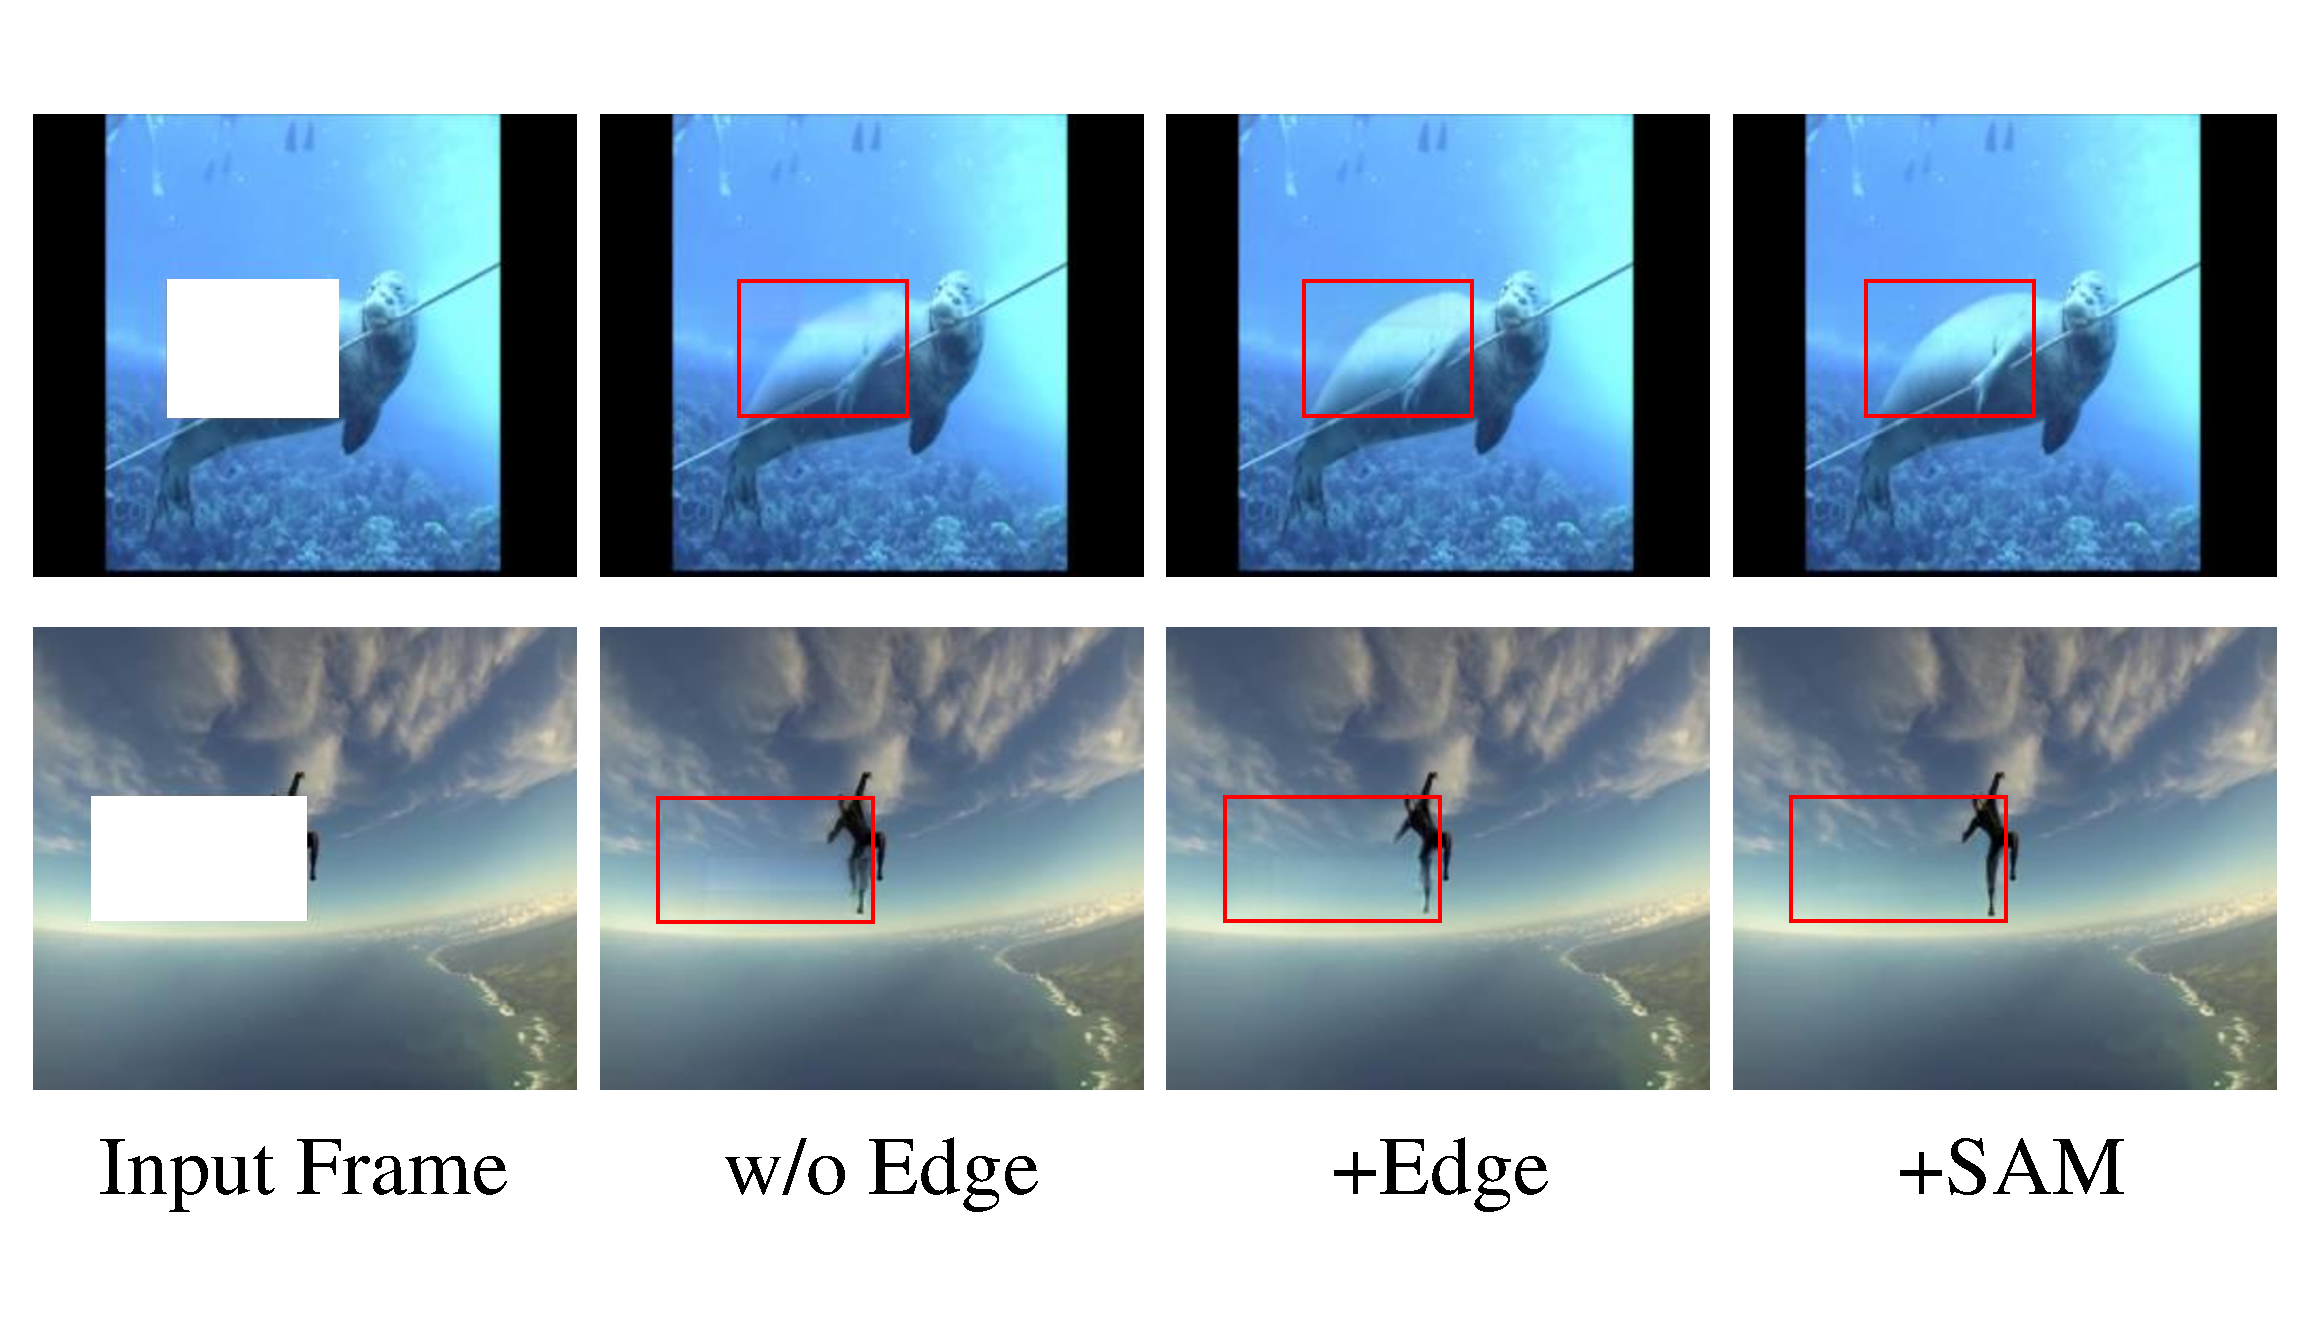
\includegraphics[width=0.97\columnwidth]{edgevis} % Reduce the figure size so that it is slightly narrower than the column. Don't use precise values for figure width.This setup will avoid overfull boxes. 
	\caption{Effects of structural guidance. By hallucinating edge maps first and then filling texture, we generate more completed and plausible target structure. Clearer boundaries can be obtained using the structure attention module.}
	\label{edgevis}
\end{figure}



In Table~\ref{tab:abl}, The model `+Edge' brings large improvement over the baseline model.
It indicates that sparse edges can provide effective structural guidance in video inpainting.
When we further add SAM, extra improvement is obtained, demonstrating that the spatial correlation between edges and textures can be better embedded and absorbed by the texture inpainting network than simply feeding the hallucinated edge maps as extra channels into TexNet.
The above analysis proves that the edge clues are effective guidance in video inpainting, which helps the network to predict more plausible frames with completed and detailed structure.
Indeed, the structure inference module ENet brings extra time cost to the baseline TexNet from 7.6335 \emph{fps} to 5.2356 \emph{fps}.
This is deserved because the inpainting quality is significantly improved.

Fig.~\ref{edgevis} shows the results generated using the three variants. 
It is obvious that after introducing structural guidance, the inpainted frames become more visually pleasing with sharper object boundaries. 
Besides, the edge maps predicted by our method are reasonable and clear, which well represent the image structure and show the strong edge inpainting ability of ENet. 
Thus, it is crucial to explore structural details in video inpainting.
 



%\begin{figure}[t]	
%    \centering
%    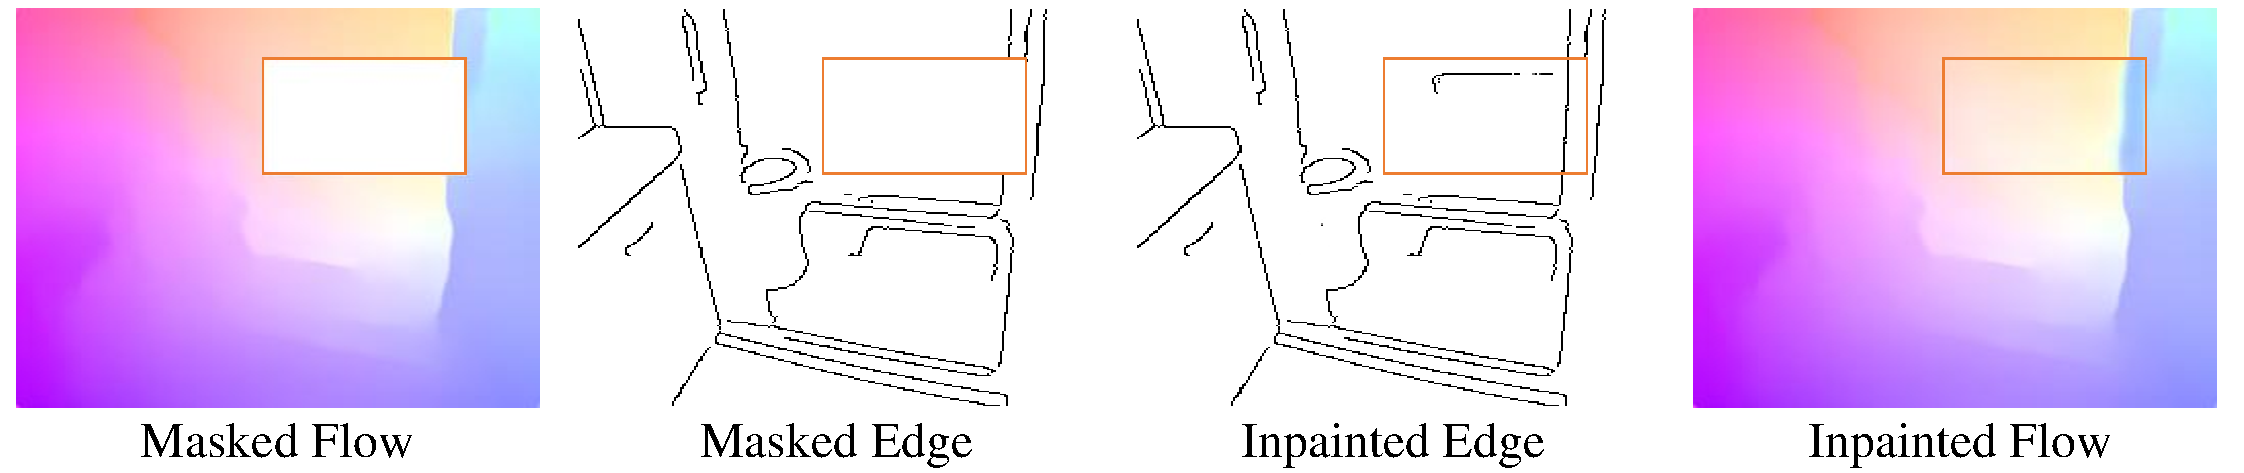
\includegraphics[width=1.0\columnwidth]{flowvis} % Reduce the figure size so that it is slightly narrower than the column. Don't use precise values for figure width.This setup will avoid overfull boxes. 
%    \caption{Visualized optical flow predicted by our method.}
%    \label{flowvis}
%\end{figure}


\begin{table}[t]
	\caption{Comparison of proposed structure attention module (SAM) and simple 2-layer spatial attention on YouTubeVOS. SAM is capable of the revealing potential correlation between structure information and video contents. }\smallskip
	\scriptsize
	\centering
	{
		\smallskip\begin{tabular}{c|c|c|c}
			\hline
			&\multicolumn{3}{c}{Free-Form Mask} \\
			\cline{2-4} 
			& PSNR & SSIM & FID\\
			
			\hline
			+Edge  &33.8206    &0.9659  &    6.6651 \\
			\hline
			
			+SimATT &34.4321    &0.9685  &   6.3125 \\
			
			\hline
			
			+SAM &\textbf{35.7783}    &\textbf{0.9712}  &   \textbf{5.8786}\\
			\hline
			
			
			
			
		\end{tabular}
	}
	\label{tab:sam_com}
\end{table}



\subsubsection{Comparison of Proposed Structure Attention Module and Simple Attention}

We propose a novel structure attention module (SAM) in TexNet to facilitate exploiting structure information of edge maps more effectively. This module is specifically designed for structural distilling in video inpainting. 
We conduct a comparison experiment between the proposed SAM and the commonly used simple 2-layer attention (SimATT) \cite{min2019two},~\emph{i.e.,} using a 2-layer convolution network to extract a spatial attention map from predicted edge maps, which is then applied to the same video feature as SAM. 
The model `+Edge' is used as the baseline.
%Compared with the SimATT, the proposed SAM considers the correlation between the edges and texture to generate the attention.
Results are shown in Table~\ref{tab:sam_com}.
The performance of SAM is better than that of SimATT. It is because that the proposed SAM is more effective in revealing potential correlation between structure information in edge maps and video contents. %Thus it is easier for TexNet to utilize structure information to obtain better results.




\begin{figure}[t]
	\centering
	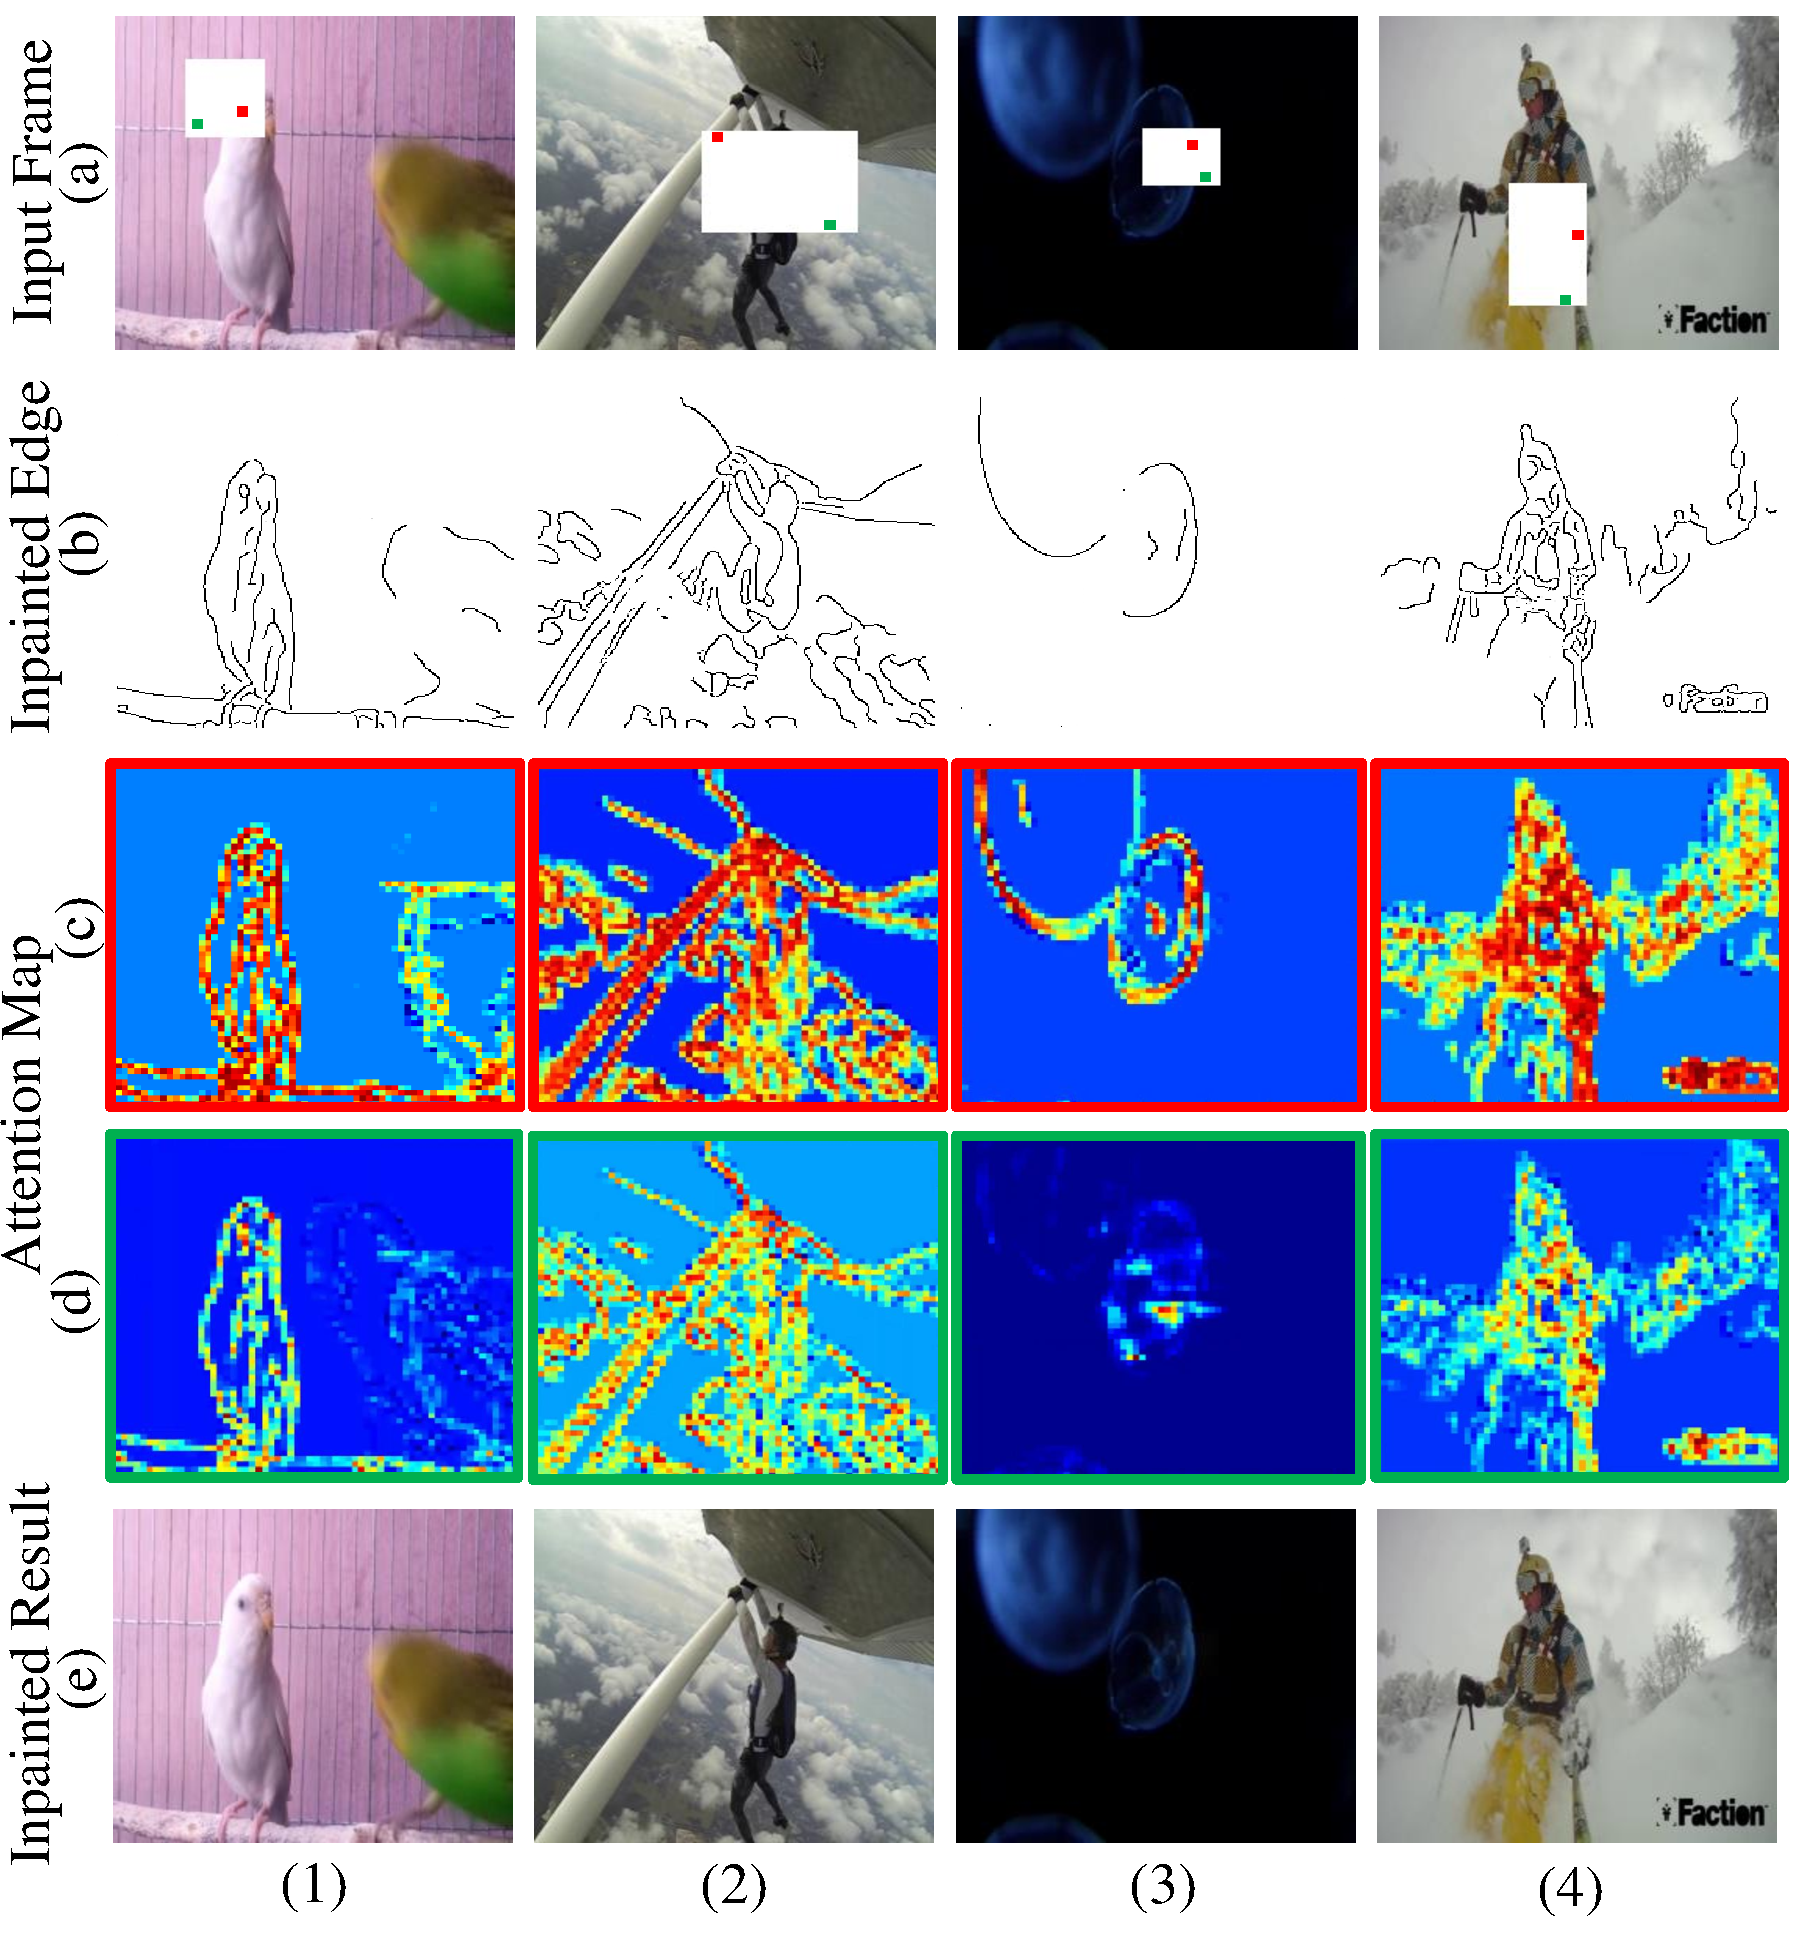
\includegraphics[width=1.0\columnwidth]{att} % Reduce the figure size so that it is slightly narrower than the column. Don't use precise values for figure width.This setup will avoid overfull boxes. 
	\caption{Visualization of the normalized attention map in proposed structure attention module. The attention map demonstrates the correlation between the selected pixel, which is denoted by red point on input frame, and all pixels on the whole input features.}
	\label{fig:att}
\end{figure}





\subsubsection{Visualization of Proposed Structure Attention Module}

To further reveal the effects of structure attention module in our framework, some visualization results are given in Fig.~\ref{fig:att}.
The red point in the input frame indicates the selected pixel to be inpainted, and the heat regions in the attention map are pixels related to that pixel.
It can be seen that, under the guidance of the edge structure, the inpainted pixel focuses on the texture around the object contours.
Thus, the generated texture in the missing regions will preserve a consistent contour according to the whole object shape, which makes the results visually reasonable.
Furthermore, the edge guidance also prevents the module from being disturbed by the background information, thus most of the heat regions are from the target and related objects.
In summary, the above observations prove that it is reasonable to introduce the edge guidance into frame inpainting, and the proposed structure attention module is an effective module in embedding the edge structure into the texture generation.








\subsubsection{Effect of Flow for Temporal Coherence}

%Temporal coherence is an important factor in video inpainting. 
We utilize temporal information to smoothen artificial flickers via two developed flow-guided warping losses during training. 
Table~\ref{tab:abl} shows that the quantitative performance is improved on all three mask settings by adding the flow guidance. Especially, we only add flow guidance in the training phase. 
Thus it brings performance gains without extra computation costs during testing.
%However, the performance improvement brought by the flow constraints is smaller than the gain caused by structural guidance.The reason is that the flow is only used in the training stage as temporal guidance, while the edge is used during the inference.
%It should be noted that predicting the completed optical flow among several frames takes more time than the edges during inference.
%Thus, we use the flow in training and the structure edge in both training and testing, which can achieve a good balance between the quality improvement and the inference efficiency. 
%
As Fig.~\ref{flow_vis} show, the synthesized contents in neighboring frames become more temporally consistent by adding the flow constrained losses.
This proves that the proposed two flow-guided constraints in edge and texture inpainting networks are effective in enhancing temporal consistency.
%and the color changes between neighboring frames become less obvious after employing flow.
%The comparison can be better illustrated in the supplementary video.
%Note that the performance gain from the temporal information is smaller than that from structure guidance in this paper.
%The reason might be that our baseline model has a certain ability to utilize complementary information from neighboring frames.

%Both the quantitative and qualitative results prove that the motion information is beneficial to temporal consistency as well as inpaitning.

 


\subsubsection{Effects of Different Hyper Parameters}
%n our experiment, we set $\lambda_1=10.0,\lambda_2=5.0$.
We conduct experiments to determine the hyper-parameters of $\lambda_1$ in Eq.~\eqref{eq:loss_e_} and $\lambda_2$ in Eq.~\eqref{eq:loss_rec}. 
We use the integration model of ENet and TexNet in this experiment without SAM and flows.
We first train ENet with different values of $\lambda_1$, and then train TexNet with restored edge maps while fixing ENet. The value of $\lambda_2$ is set as $0.2$ when testing different $\lambda_1$.
When determining $\lambda_2$ for TexNet, we set $\lambda_1=10.0$.

$\lambda_1$ is used in Eq.~\eqref{eq:loss_e_} as a weight of feature matching loss when training ENet. %The quality of generated edge maps should be measured by the quantitative results of inpainted frames in task of video inpainting. 
%Thus, 
From the curve in Fig.~\ref{fig:hparam}, when increasing $\lambda_1$ from $0.0$ to $2.0$, the performance gain is obvious, which proves that the feature matching loss is effective in
generating high-quality edge maps used for the final inpainted results. 
Then when $\lambda_1$ is increased from $2.0$ to $10.0$, slight improvement is obtained.
The model obtains the best performance at $\lambda_1=10.0$.
%Therefore, we set $\lambda_1$ to $10.0$ for the experimental settings.
%
$\lambda_2$ in Eq.~\eqref{eq:loss_rec} is the weight of $l_1$-reconstruction loss of the coarse prediction in TexNet. 
When $\lambda_2$ is $0.0$, the TexNet is trained without supervision of the coarse prediction, and the inpainting quality is significantly harmed.
% the result is heavily harmed. 
It demonstrates that the coarse-to-fine architecture is effective in TexNet. The best performance is obtained when $\lambda_2=0.2$. And performance drops when $\lambda_2>0.2$, which reflects that the supervision on the fine prediction networks is more important.
Therefore, we set $\lambda_2$ as $0.2$ in all the other experiments.
%Results are shown in Fig.~\ref{fig:hparam}. As shown, $\lambda_1=10.0,\lambda_2=5.0$ is the best choice.


\begin{figure}[t]
	\centering
	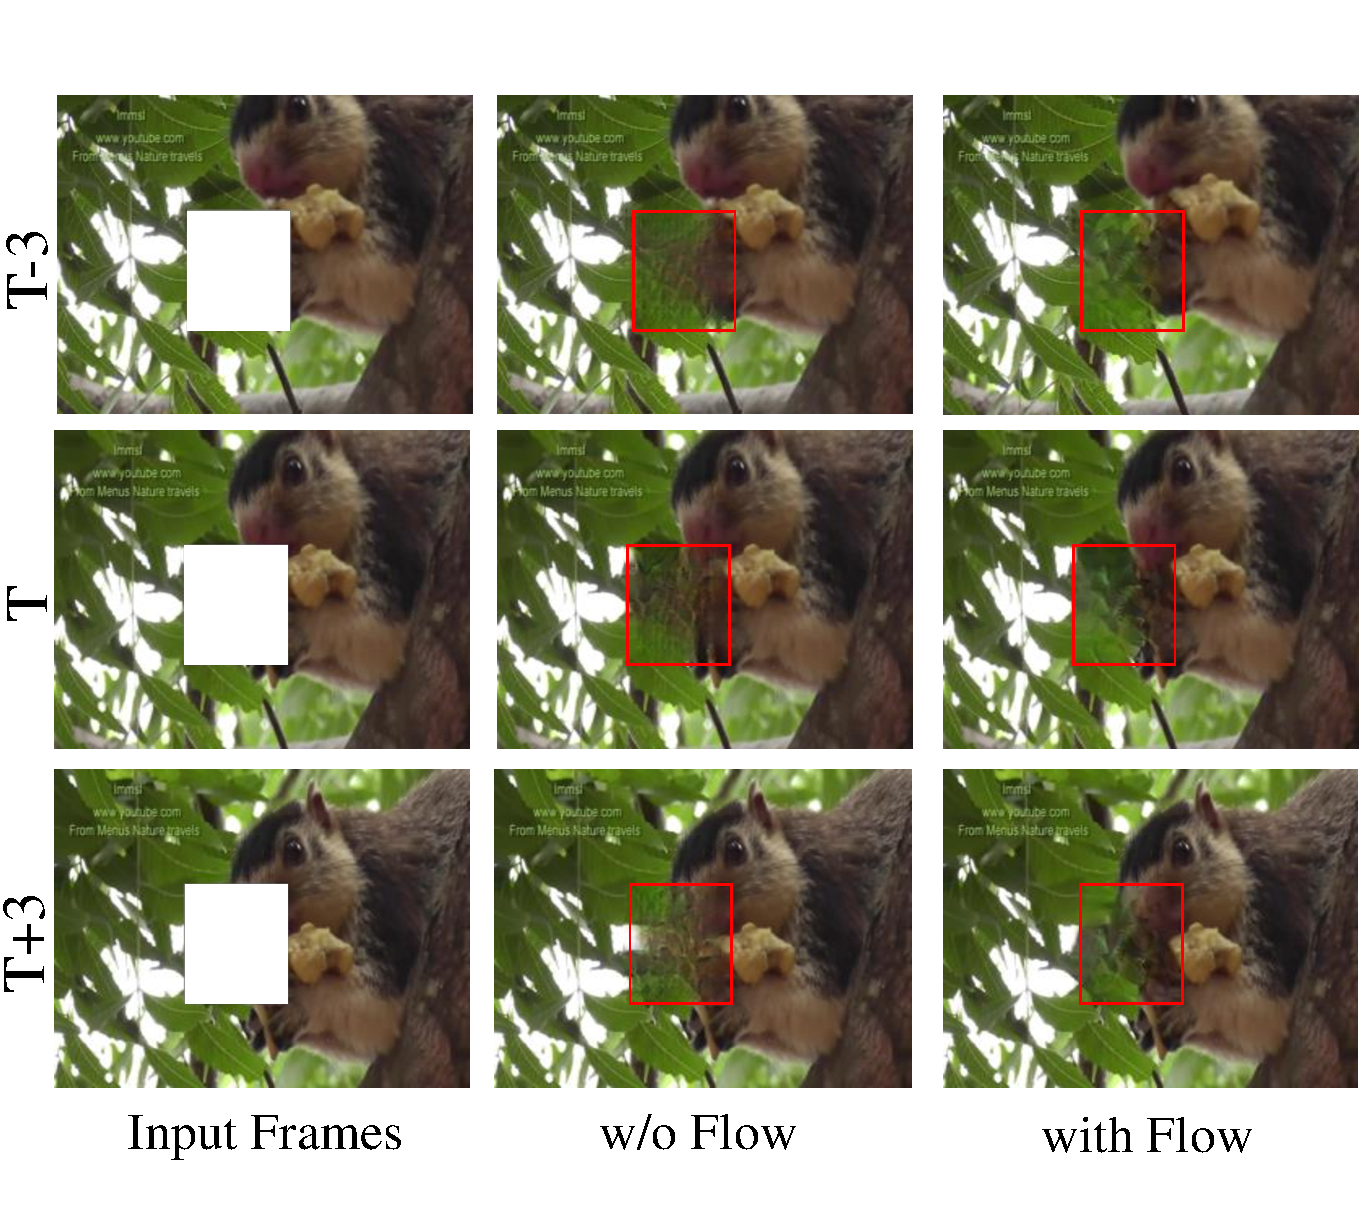
\includegraphics[width=0.9\columnwidth]{flow_vis} % Reduce the figure size so that it is slightly narrower than the column. Don't use precise values for figure width.This setup will avoid overfull boxes. 
	\caption{Inpainting results of three neighboring frames. With the flow constraints during network training, the inpainting results are more temporally consistent without introducing image blurs. }
	\label{flow_vis}
\end{figure}



\begin{figure}[t]
	\centering
	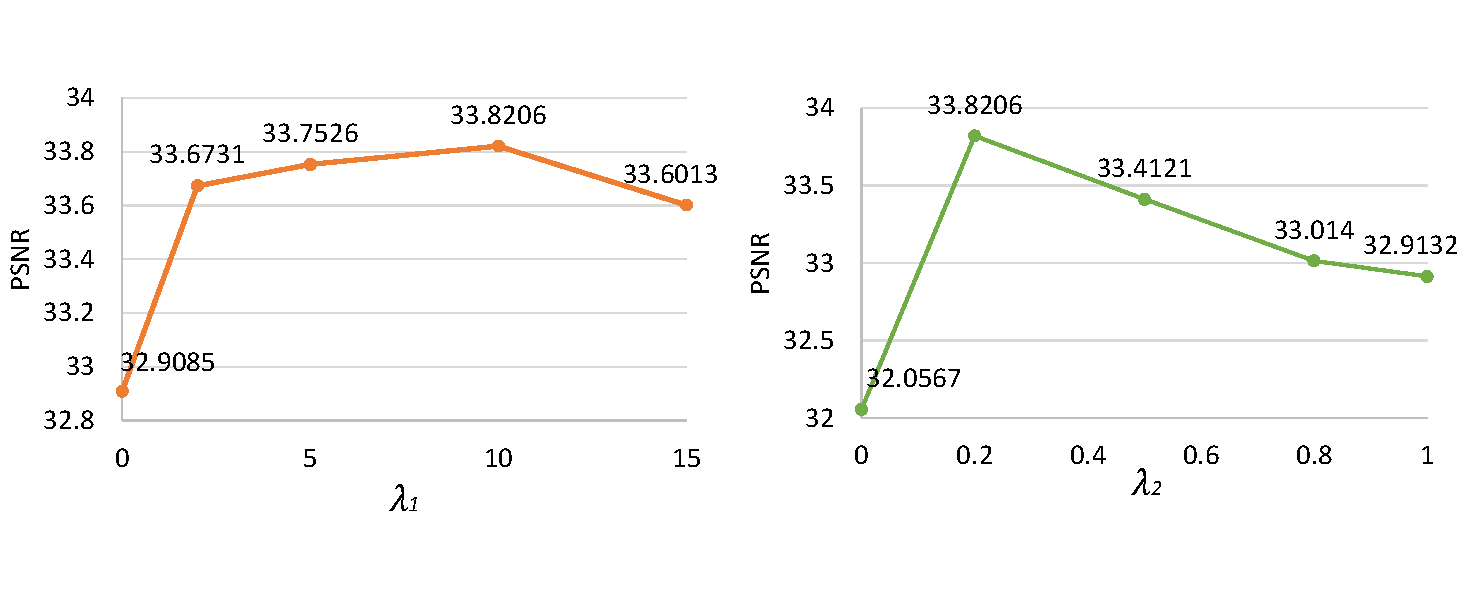
\includegraphics[width=1.0\columnwidth]{lamda1} % Reduce the figure size so that it is slightly narrower than the column. Don't use precise values for figure width.This setup will avoid overfull boxes. 
	\caption{Comparison of hyper parameters $\lambda_1$ and $\lambda_2$. The best result is obtained when $\lambda_1=10.0$ and $\lambda_2=0.2$.}
	\label{fig:hparam}
\end{figure}






 





\section{Conclusion}\label{sec:conclu}
In this paper, we propose a novel structure-guided video inpainting approach, which effectively utilizes structure information to generate fine-detailed frames.
The edges in the missing region are first estimated to represent the target structure explicitly, using an edge inpainting network. 
Then under the guidance of the sparse edges, the missing content can be synthesized with intact structure and fine details.
%
Our proposed structure attention module effectively exploits the correlation between structure and textures to improve visual quality.
%
Besides, the temporal coherence of the inpainting frames is further enhanced by our flow-assisted losses.
Experiments on YouTubeVOS and DAVIS datasets demonstrate the effectiveness of our method.





% use section* for acknowledgment
%\section*{Acknowledgment}
%This work was supported by the National Key Research and Development Program of China (2017YFC0820600), the National Natural Science Foundation of China under Nos. 61525206, 61472377, 61632006, 91732304, and 61771468,the Fundamental Research Funds for the Central Universities under Grant WK2380000002, National Defense Science and Technology Fund for Distinguished Young Scholars (2017-JCJQ-ZQ-022), the Youth Innovation Promotion Association Chinese Academy of Sciences (2017209).


% Can use something like this to put references on a page
% by themselves when using endfloat and the captionsoff option.
\ifCLASSOPTIONcaptionsoff
  \newpage
\fi



% trigger a \newpage just before the given reference
% number - used to balance the columns on the last page
% adjust value as needed - may need to be readjusted if
% the document is modified later
%\IEEEtriggeratref{8}
% The "triggered" command can be changed if desired:
%\IEEEtriggercmd{\enlargethispage{-5in}}

% references section

% can use a bibliography generated by BibTeX as a .bbl file
% BibTeX documentation can be easily obtained at:
% http://mirror.ctan.org/biblio/bibtex/contrib/doc/
% The IEEEtran BibTeX style support page is at:
% http://www.michaelshell.org/tex/ieeetran/bibtex/
\bibliographystyle{IEEEtran}
% argument is your BibTeX string definitions and bibliography database(s)
\bibliography{ref}
%
% <OR> manually copy in the resultant .bbl file
% set second argument of \begin to the number of references
% (used to reserve space for the reference number labels box)




% that's all folks
\end{document}


